%% draft_pcycle_basins.tex
%% Draft research article — November 2026
%% Authors: V. Álvarez-Aparicio, J.M. García-Calcines,
%%          L.J. Hernández-Paricio, M.T. Rivas-Rodríguez
%%
%% Compile: pdflatex draft_pcycle_basins.tex (twice)
%%          bibtex  draft_pcycle_basins
%%          pdflatex draft_pcycle_basins.tex (twice more)

\documentclass[12pt]{article}

\usepackage{amsmath, amssymb, amsthm}
\usepackage{mathtools}
\usepackage{geometry}
\geometry{a4paper, margin=2.5cm}
\usepackage{hyperref}
\usepackage{enumitem}
\usepackage{microtype}
\usepackage{algorithm}
\usepackage{algpseudocode}
\usepackage{xcolor}
\usepackage{graphicx}
\usepackage{booktabs}

%% ---- Theorem environments ------------------------------------------------
\newtheorem{theorem}{Theorem}[section]
\newtheorem{proposition}[theorem]{Proposition}
\newtheorem{lemma}[theorem]{Lemma}
\newtheorem{corollary}[theorem]{Corollary}
\newtheorem{conjecture}[theorem]{Conjecture}
\theoremstyle{definition}
\newtheorem{definition}[theorem]{Definition}
\newtheorem{example}[theorem]{Example}
\newtheorem{remark}[theorem]{Remark}

%% ---- Macros ---------------------------------------------------------------
\newcommand{\C}{\mathbb{C}}
\newcommand{\R}{\mathbb{R}}
\newcommand{\Z}{\mathbb{Z}}
\newcommand{\N}{\mathbb{N}}
\newcommand{\Q}{\mathbb{Q}}
\newcommand{\Chat}{\hat{\C}}
\newcommand{\Pone}{\mathbf{P}^1(\C)}
\newcommand{\Poneplus}{\mathbf{P}^{1+}(\C)}
\newcommand{\fsh}{f^{\#}}
\newcommand{\Ff}{F(f)}
\newcommand{\Jf}{J(f)}
\newcommand{\Bf}{B_f}
\newcommand{\Bfp}{B_f^{(p)}}
\newcommand{\Bfzero}{B_f^0}
\newcommand{\hpair}{[F:G]}
\newcommand{\sgn}{\operatorname{sgn}}
\DeclareMathOperator{\Arg}{Arg}
\DeclareMathOperator{\Wron}{Wr}
\DeclareMathOperator{\ord}{ord}

%% ---------------------------------------------------------------------------
\title{\textbf{Basins of Attraction of Periodic Orbits\\
        of Rational Maps on the Riemann Sphere:\\
        Algorithms, Bounds, and Visualizations}\\[6pt]
       {\large (Working draft --- November 2026)}}

\author{V.~\'Alvarez-Aparicio\thanks{Departamento de Matem\'aticas y
Computaci\'on, Universidad de La Rioja, Logro\~no, Spain.} \and
J.\,M.~Garc\'ia-Calcines\thanks{Departamento de Matem\'aticas,
Estad\'istica e I.O., Universidad de La Laguna, Spain.} \and
L.\,J.~Hern\'andez-Paricio\footnotemark[1] \and
M.\,T.~Rivas-Rodr\'iguez\footnotemark[1]}

\date{November 2026}

\begin{document}

\maketitle

%% ---------------------------------------------------------------------------
\begin{abstract}
We study the basins of attraction of periodic attracting and superattracting
orbits of rational self-maps $f\colon\Pone\to\Pone$ of degree $d\geq 2$,
using homogeneous coordinates throughout so that the point at infinity is
treated on equal footing with finite points.  A central tool is the
\emph{spherical derivative} $\fsh$, whose geometric mean around a periodic
orbit gives the \emph{Lyapunov constant} $c$; a cycle is attracting when
$c<1$ and superattracting when $c=0$.

Our main contributions are threefold.  First, we provide a self-contained
algorithmic framework for locating and classifying all attracting $p$-cycles
(periodic orbits of minimal period~$p$) and their basins in $\Pone$, based
on the homogeneous model and the chordal metric.  Second, we prove and exploit
Fatou's critical-orbit theorem: every attracting cycle attracts at least one
of the $2d-2$ critical points of~$f$, yielding a sharp and effectively
computable upper bound~$P$ on the maximal attracting period.  Third, we
implement these algorithms in the Julia package \texttt{RiemannBasins.jl}
and illustrate them on several families of rational maps, including the
quadratic family $z^2+c$, Newton's method for polynomials, and Halley's
method.

The connection between the Wronskian of the homogeneous pair $(F,G)$ and the
correct two-chart formula for $\fsh$ is discussed in detail; a subtle sign
issue with the standard single-chart formula near $\infty$ is identified and
corrected.
\end{abstract}

\tableofcontents

%% ===========================================================================
\section{Introduction}
\label{sec:intro}
%% ===========================================================================

The dynamics of rational maps on the Riemann sphere is one of the central
topics of one-dimensional complex analysis.  The Fatou set $\Ff$ of a
rational map $f$ of degree $d\geq 2$ is the maximal open subset of
$\Chat = \C\cup\{\infty\}$ on which the family of iterates
$\{f^n\}_{n\geq 0}$ is locally equicontinuous; its complement $\Jf$ is
the Julia set.  By Sullivan's No-Wandering-Domain theorem \cite{Sullivan1985},
every connected component of $\Ff$ is eventually periodic, and the periodic
Fatou components fall into exactly five types: attracting basins,
superattracting basins, parabolic basins, Siegel discs, and Herman rings
\cite{Milnor2006}.

Among these, the \emph{attracting and superattracting basins} are both the
most common in practice and the most amenable to algorithmic computation,
because the orbit of any point in such a basin converges geometrically (or
super-geometrically) to the attracting cycle.  Given a $p$-cycle
$\Gamma = \{z_0, z_1=f(z_0), \ldots, z_{p-1}=f^{p-1}(z_0)\}$ with
$f(z_{p-1})=z_0$, the \emph{basin of attraction}
$\Bf(\Gamma) = \{z\in\Pone : f^{np}(z)\to\Gamma\}$ decomposes into
$p$ pairwise disjoint $f$-invariant open sets $B_{z_k}$, one for each cycle
point~$z_k$; each~$B_{z_k}$ may itself have infinitely many connected
components (the cycle point, all its preimages under $f^p$, preimages of
preimages, etc.).  The \emph{immediate basin} $B^0_{z_k}$ is the connected
component of~$B_{z_k}$ that contains $z_k$ itself.  The map $f$ sends
$B^0_{z_k}$ onto $B^0_{z_{k+1\bmod p}}$, so the $p$ immediate basin
components form a single cycle of simply connected domains.

The key practical question is: \emph{how do we find all attracting cycles and
their basins, and how many iterations suffice?}  Fatou's theorem
\cite{Fatou1919,Fatou1920} provides the answer: the immediate basin
$B^0_{z_0}\cup\cdots\cup B^0_{z_{p-1}}$ of every attracting cycle contains
at least one \emph{critical point} of~$f$ (a zero of the Wronskian
$\Wron(F,G) = F'G - FG'$ in homogeneous coordinates).  Since $f$ has at
most $2d-2$ critical points, it can have at most $2d-2$ distinct attracting
or superattracting cycles, and tracing the orbit of each critical point
reveals every such cycle.

Our implementation in the Julia package \texttt{RiemannBasins.jl}
\cite{RiemannBasins} exposes this theory through two related function groups.
The first, \texttt{basin\_portrait\_pcycle}, visualises the basin of every
$p$-cycle for a user-supplied period $p$.  The second, the
\texttt{critical\_orbit\_analysis} family (§14 of the package), implements
Fatou's theorem directly: it computes the Wronskian roots, traces each
critical orbit, detects the period of the attracting cycle reached, computes
the Lyapunov constant~$c$, and returns a sharp upper bound~$P$ via
\texttt{max\_attracting\_period}.
The Lyapunov-based cycle-detection strategy originates in the theoretical
framework of \cite{AlvarezAparicio2023} and was first prototyped in
\texttt{LCD.jl}~\cite{LCD2022}; a further application to the dynamical study
of Chebyshev's method on polynomials appears in~\cite{AlvarezAparicio2023MMEHB}.

The topological structure of the Julia set $\Jf$ provides an independent
perspective on the fractal geometry underlying the basin boundaries studied
here.  For an expanding rational map, the shape of $\Jf$---in the sense of
Marde\v{s}i\'c--Segal shape theory---is captured by an inverse system of
cubic complexes built from the global (spherical) multiplier; the resulting
shape invariants and the $d$-fold self-overlay structure of the restriction
$f|_{\Jf}\colon\Jf\to\Jf$, together with its symmetries encoded via the
fundamental pro-groupoid in the symmetric group $\Sigma_d$, are studied
in~\cite{Extremiana2018Shape,Extremiana2018SelfOverlays}.

Several Julia packages for complex dynamics visualisation already exist,
most notably \texttt{Fatou.jl} \cite{FatouJl}, which accepts arbitrary
complex maps (including transcendental ones) and produces richly coloured
escape-time and orbit-trap portraits with GPU acceleration.
\texttt{RiemannBasins.jl} differs in three respects.
First, it works on the full Riemann sphere $\Pone$ in homogeneous
coordinates, so the point $\infty=[1:0]$ is a regular point with its own
basin and its own affine chart, rather than a mere escape threshold.
Second, it implements Fatou's critical-orbit theorem
(Theorem~\ref{thm:fatou}) algorithmically: given the homogeneous pair
$\hpair$, the package locates \emph{all} attracting cycles automatically
via Wronskian root-finding, computes their Lyapunov constants, and returns
a provably sharp upper bound~$P$ on the maximum attracting period.
Third, its \texttt{pcycle\_lch} colour strategy encodes the cyclic
structure of the basin decomposition---which cycle, which sub-basin within
that cycle, and how fast---using a perceptually uniform
$\mathrm{LCH}_{ab}$ scheme, making the cyclic permutation
$f\colon B_j\to B_{j+1\bmod p}$ directly readable from the image
(Section~\ref{sec:colour}).

The paper is organised as follows.
Section~\ref{sec:prelim} reviews the homogeneous model for $\Pone$, the
chordal metric, and the spherical derivative in both affine charts.
Section~\ref{sec:periodic} defines $p$-cycles, their Lyapunov stability, and
the classification into attracting/superattracting/indeterminate orbits.
Section~\ref{sec:fatou} summarises the relevant theory of Fatou components and
states Fatou's critical-orbit theorem.
Section~\ref{sec:algorithms} presents the two main algorithms in full
pseudocode.
Section~\ref{sec:examples} illustrates the algorithms on four families of
maps.
Section~\ref{sec:discussion} discusses open problems and extensions.

%% ===========================================================================
\section{Preliminaries: the Riemann sphere in homogeneous coordinates}
\label{sec:prelim}
%% ===========================================================================

\subsection{The projective line $\Pone$}

We model the Riemann sphere as the \emph{complex projective line}
\[
  \Pone = \bigl(\C^2\setminus\{(0,0)\}\bigr)\big/{\sim},
  \qquad
  (z,t)\sim(\lambda z,\lambda t),\quad \lambda\in\C^*,
\]
writing a point as a homogeneous pair $[z:t]$.  The affine chart
$\{t\neq 0\}$ is identified with $\C$ via $[z:t]\mapsto z/t$, and the
point $[1:0]$ represents $\infty$.  We work with \emph{normalised}
representatives: given $(z,t)\neq(0,0)$, define
\begin{equation}\label{eq:normalize}
  \nu(z,t) =
  \begin{cases}
    (z/t,\;1)   & \text{if }|t|\geq|z|,\\[2pt]
    (1,\;t/z)   & \text{if }|z|>|t|.
  \end{cases}
\end{equation}
The first case gives coordinates in the standard affine chart
$(\zeta,1)$ with $|\zeta|\leq 1$; the second gives coordinates in the
second chart $(1,w)$ with $|w|<1$.

\subsection{Chordal metric}

The \emph{chordal metric} on $\Pone$ is
\begin{equation}\label{eq:chordal}
  \sigma\bigl([z_1:t_1],[z_2:t_2]\bigr)
  = \frac{2\,|z_1\bar t_2 - z_2\bar t_1|}%
         {\sqrt{(|z_1|^2+|t_1|^2)(|z_2|^2+|t_2|^2)}}.
\end{equation}
It satisfies $0\leq\sigma\leq 2$, with $\sigma=2$ iff one point is $0=[0:1]$
and the other is $\infty=[1:0]$.  On normalised representatives
$\nu(z,t)=(\zeta,1)$, formula~\eqref{eq:chordal} reduces to the standard
spherical distance
$\sigma([\zeta_1:1],[\zeta_2:1]) = 2|\zeta_1-\zeta_2|/\sqrt{(1+|\zeta_1|^2)(1+|\zeta_2|^2)}$.

\subsection{Rational maps in homogeneous coordinates}

A rational map $f\colon\Pone\to\Pone$ of degree $d\geq 1$ is given by a
\emph{homogeneous pair} $\hpair$ of polynomials
\begin{align}
  F(z,t) &= \sum_{k=0}^d a_k\, z^k\, t^{d-k},\quad
             a_k\in\C,
  \label{eq:Fpoly}\\
  G(z,t) &= \sum_{k=0}^d b_k\, z^k\, t^{d-k},\quad
             b_k\in\C,
  \label{eq:Gpoly}
\end{align}
where $F$ and $G$ have no common homogeneous factor, and
$f([z:t]) = [F(z,t):G(z,t)]$.  We adopt the \emph{constant-first}
convention: the coefficient list is $[a_0,a_1,\ldots,a_d]$ so that
$a_0$ is the constant term (coefficient of $t^d$) and $a_d$ is the
leading term (coefficient of $z^d$).  Under the affine identification
$[z:1]\leftrightarrow z$, the map becomes $f(z)=p(z)/q(z)$ where
$p(z)=F(z,1)=\sum_k a_k z^k$ and $q(z)=G(z,1)=\sum_k b_k z^k$.

\begin{remark}
When $\deg p\neq\deg q$, one polynomial is padded with leading zero
coefficients until both have degree $d=\max(\deg p,\deg q)$.
This ensures both $F$ and $G$ are homogeneous of the same degree, and in
particular that $f(\infty)=[a_d:b_d]$ is well defined.
\end{remark}

\subsection{Spherical derivative --- two-chart formula}
\label{subsec:sphderiv}

The \emph{spherical derivative} of $f$ at $[z:t]\in\Pone$ measures the
local expansion in the chordal metric.  In the affine chart ($|t|\geq|z|$,
$u=z/t$) it equals
\begin{equation}\label{eq:sphderiv_affine}
  \fsh(u) = \frac{|f'(u)|\,(1+|u|^2)}{1+|f(u)|^2},
\end{equation}
while in the second chart ($|z|>|t|$, $w=t/z$) it equals
$\fsh = g^{\#}(w)$ for $g(w)=1/f(1/w)$.

In homogeneous coordinates, let
\begin{align*}
  W_z(z,t) &= \frac{\partial F}{\partial z}\,G - F\,\frac{\partial G}{\partial z},
  &
  W_t(z,t) &= \frac{\partial F}{\partial t}\,G - F\,\frac{\partial G}{\partial t}.
\end{align*}
Both are homogeneous of degree $2d-1$.  Euler's identity for homogeneous
functions gives $z\,\partial F/\partial z + t\,\partial F/\partial t = d\,F$,
from which one derives
\begin{equation}\label{eq:Wrel}
  W_t(z,t) = -\frac{z}{t}\,W_z(z,t), \qquad t\neq 0.
\end{equation}

\begin{proposition}[Two-chart spherical derivative]\label{prop:sphderiv}
For any normalised representative $\nu(z,t)$ of a point
$[z:t]\in\Pone$,
\begin{equation}\label{eq:sphderiv_hom}
  \fsh([z:t]) =
  \begin{cases}
    \dfrac{|W_z(z,t)|}{|t|\,(|F(z,t)|^2+|G(z,t)|^2)}\,(|z|^2+|t|^2)
      & \text{if }|t|\geq|z|, \\[10pt]
    \dfrac{|W_t(z,t)|}{|z|\,(|F(z,t)|^2+|G(z,t)|^2)}\,(|z|^2+|t|^2)
      & \text{if }|z|>|t|.
  \end{cases}
\end{equation}
For normalised representatives ($\max(|z|,|t|)=1$) the denominators
$|t|$ and $|z|$ both equal $1$, so the formula simplifies to
$\fsh = |W_{\mathrm{chart}}|\,(|z|^2+|t|^2)/(|F|^2+|G|^2)$.
\end{proposition}

\begin{proof}
In the first chart, $t=1$, $u=z$ and
$W_z(u,1) = p'(u)q(u)-p(u)q'(u)$ is the affine Wronskian.
By homogeneity of degree $2d-1$, $W_z(z,t)=t^{2d-1}W_z(z/t,1)$.
Substituting into~\eqref{eq:sphderiv_affine} and simplifying yields the
first case.  The second case follows by applying the first case to $g(w)$
in the second chart.
\end{proof}

\begin{remark}\label{rem:chartbug}
Using $W_z$ in both charts (as in a naive single-formula implementation)
gives the correct value for first-chart points but returns $0$ for
points of the form $[1:0]$ (the point $\infty$) due to~\eqref{eq:Wrel}:
$W_z(1,0) = 0$ whenever the leading coefficients of $F$ and $G$
conspire to make $W_z$ vanish there, while $W_t(1,0)$ correctly
captures the derivative in the second chart.  An implementation must
therefore branch on the chart; see Section~\ref{sec:algorithms} and
the note in \texttt{RiemannBasins.jl} \S14.
\end{remark}

%% ===========================================================================
\section{Periodic orbits and their stability}
\label{sec:periodic}
%% ===========================================================================

\subsection{$p$-Cycles}

\begin{definition}\label{def:pcycle}
A point $z_0\in\Pone$ is \emph{periodic} of \emph{(minimal) period} $p\geq 1$
under $f$ if $f^p(z_0)=z_0$ and $f^k(z_0)\neq z_0$ for $1\leq k<p$.
The set $\Gamma_p = \{z_0, z_1,\ldots,z_{p-1}\}$ with $z_k=f^k(z_0)$ is
called a \emph{$p$-cycle}.  A periodic point of period~$1$ is a \emph{fixed
point}.
\end{definition}

Equivalently, the points $z_0,\ldots,z_{p-1}$ are the fixed points of $f^p$
that are \emph{not} fixed points of $f^k$ for any proper divisor $k\mid p$
with $k<p$.

\begin{remark}[Counting $p$-cycles]
The number of fixed points of $f^p$ in $\Pone$ is $d^p+1$ (counted with
multiplicity, by B\'ezout's theorem applied to the homogeneous system
$F_p(z,t)=\lambda\,z$, $G_p(z,t)=\lambda\,t$).  By M\"obius inversion, the
number of periodic points of exact minimal period $p$ is
$\sum_{k|p}\mu(p/k)(d^k+1)$, where $\mu$ is the M\"obius function.
\end{remark}

\subsection{Stability and the Lyapunov constant}

The classical stability criterion for a $p$-cycle $\Gamma_p$ uses the
\emph{multiplier}
\begin{equation}\label{eq:multiplier}
  \lambda(\Gamma_p) = (f^p)'(z_0) = \prod_{k=0}^{p-1} f'(z_k),
\end{equation}
computed in the affine chart (or via the Schwarzian derivative near $\infty$).
The cycle is \emph{attracting} if $|\lambda|<1$,
\emph{superattracting} if $\lambda=0$,
\emph{repelling} if $|\lambda|>1$, and
\emph{indifferent} if $|\lambda|=1$.

For numerical and algorithmic purposes, the \emph{Lyapunov constant}
\cite{AlvarezAparicio2023}
\begin{equation}\label{eq:lyapunov}
  c(\Gamma_p) = \biggl(\prod_{k=0}^{p-1}\fsh(z_k)\biggr)^{1/p}
\end{equation}
is more convenient, as it uses the chart-independent spherical derivative
$\fsh$ and is defined uniformly for all cycle points including $\infty$.

\begin{proposition}\label{prop:lyapunov_vs_multiplier}
Let $\Gamma_p=\{z_0,\ldots,z_{p-1}\}$ be a $p$-cycle with all points in
the affine chart $\{t\neq 0\}$.  Then
\[
  c(\Gamma_p)^p = |\lambda(\Gamma_p)|\cdot
                   \frac{\prod_k (1+|z_k|^2)}%
                        {\prod_k (1+|f(z_k)|^2)}.
\]
Since $f(z_{k})=z_{k+1}$ (cyclically), the last ratio equals $1$, and
therefore $c(\Gamma_p) = |\lambda(\Gamma_p)|^{1/p}$.
\end{proposition}

The proposition shows that $c<1\Leftrightarrow|\lambda|<1$,
$c=0\Leftrightarrow\lambda=0$, etc., so the Lyapunov constant carries
the same stability information as the multiplier, but is well-defined
at $\infty$ and throughout $\Pone$.

\begin{definition}\label{def:classification}
Let $c=c(\Gamma_p)$ be the Lyapunov constant of a $p$-cycle.
\begin{itemize}[noitemsep]
  \item $c=0$: \emph{superattracting} cycle.
  \item $0<c<1$: \emph{attracting} cycle.
  \item $c\geq 1$ (after numerical warmup): \emph{indeterminate}
        (may be repelling, indifferent, or the warmup was insufficient).
\end{itemize}
\end{definition}

The threshold $c<1$ requires a numerical tolerance; in practice, we use
$c<\varepsilon_{\mathrm{attr}}=1-10^{-6}$ for attracting and
$c<10^{-8}$ for superattracting.

\subsection{Superattracting cycles and critical points}

A cycle $\Gamma_p$ is superattracting if and only if at least one cycle
point $z_k$ satisfies $f'(z_k)=0$, i.e., $z_k$ is a \emph{critical point}
of $f$.  In this case the spherical derivative $\fsh(z_k)=0$, so the product
in~\eqref{eq:lyapunov} vanishes.

\begin{definition}\label{def:critical}
A point $z_0=[z:t]\in\Pone$ is a \emph{critical point} of $f=\hpair$ of
degree $d$ if
\[
  W_z(z,t) = \frac{\partial F}{\partial z}(z,t)\,G(z,t)
            - F(z,t)\,\frac{\partial G}{\partial z}(z,t) = 0.
\]
(If additionally $|z|>|t|$, one uses $W_t$ instead; see
Proposition~\ref{prop:sphderiv}.)
\end{definition}

The polynomial $W_z(z,1) = p'(z)q(z)-p(z)q'(z)$ has degree at most
$2d-2$, so there are at most $2d-2$ finite critical points.  The point
$\infty=[1:0]$ is a critical point if and only if $\deg(W_z)<2d-2$,
equivalently if the leading coefficient of $W_z(z,1)$ vanishes, which
happens when $f$ has a critical point at $\infty$ in the second-chart
sense.

%% ===========================================================================
\section{Fatou components and basins of $p$-cycles}
\label{sec:fatou}
%% ===========================================================================

\subsection{The Fatou and Julia decomposition}

\begin{definition}
The \emph{Fatou set} $\Ff$ of $f$ is the set of points $z\in\Pone$
having a neighbourhood $U$ on which $\{f^n|_U\}$ is a normal family
(in the sense of Montel).  Its complement $\Jf=\Pone\setminus\Ff$ is
the \emph{Julia set}.
\end{definition}

Both $\Ff$ and $\Jf$ are completely invariant: $f^{-1}(\Ff)=\Ff$ and
$f^{-1}(\Jf)=\Jf$.  For $d\geq 2$ the Julia set is a non-empty perfect
set (compact with no isolated points) \cite{Milnor2006}.
The topological \emph{shape} of $\Jf$, studied via inverse systems of
cubic complexes built from the spherical multiplier, is analysed
in~\cite{Extremiana2018Shape,Extremiana2018SelfOverlays}.

\begin{theorem}[Sullivan, 1985 \cite{Sullivan1985}]
Every connected component $U$ of $\Ff$ is eventually periodic: there
exist $n_0,m\geq 0$ with $f^{n_0+m}(U)\subseteq f^{n_0}(U)$.
\end{theorem}

Periodic Fatou components are classified into five types:
\begin{enumerate}[label=(\roman*)]
  \item \textbf{Attracting basin}: contains an attracting cycle point.
  \item \textbf{Superattracting basin}: contains a superattracting cycle
        point.
  \item \textbf{Parabolic basin}: boundary contains an indifferent cycle
        with $\lambda=e^{2\pi i p/q}$ a root of unity.
  \item \textbf{Siegel disc}: biholomorphic to a disc; $f$ acts as an
        irrational rotation.
  \item \textbf{Herman ring}: biholomorphic to an annulus; $f$ acts as an
        irrational rotation.
\end{enumerate}

\subsection{Basins of $p$-cycles}

\begin{definition}\label{def:basin}
Let $\Gamma_p=\{z_0,\ldots,z_{p-1}\}$ be an attracting or superattracting
$p$-cycle.  The \emph{basin of attraction} of $\Gamma_p$ is
\begin{equation}\label{eq:basin}
  \Bf(\Gamma_p) = \bigl\{z\in\Pone : \sigma(f^{np}(z),\Gamma_p)\to 0
                           \text{ as }n\to\infty\bigr\}.
\end{equation}
The \emph{immediate basin} of $z_k$ is the connected component $B^0_{z_k}$
of $\Bf(\Gamma_p)$ containing $z_k$.
\end{definition}

The full basin is the disjoint union $\Bf(\Gamma_p)=\bigsqcup_{k=0}^{p-1}
B_{z_k}$ where $B_{z_k}=\{z:\sigma(f^{np+k}(z),z_k)\to 0\}$; note that
$f$ maps $B_{z_k}$ to $B_{z_{k+1}}$ (indices mod $p$).
The spherical measure (probability) of these basins on $S^2$, and its
dependence on the relaxation parameter, was studied quantitatively
in~\cite{Gutierrez2016Measures}.

\begin{theorem}[Fatou, 1919--1920 \cite{Fatou1919,Fatou1920}]
\label{thm:fatou}
Let $f$ be a rational map of degree $d\geq 2$ and let $\Gamma_p$ be an
attracting or superattracting $p$-cycle with immediate basins
$B^0_{z_0},\ldots,B^0_{z_{p-1}}$.  At least one immediate basin component
$B^0_{z_k}$ contains a critical point of~$f$; equivalently, at least one
critical point of~$f$ is attracted to~$\Gamma_p$.  (For superattracting
cycles, every $z_k$ is itself a critical point of~$f$, so each $B^0_{z_k}$
contains one; for merely attracting cycles, at least one component
suffices.)
\end{theorem}

\begin{proof}[Proof sketch]
Fix one immediate basin component $B^0_{z_0}$ and consider the iterate
$g = f^p\colon B^0_{z_0}\to B^0_{z_0}$, which has an attracting fixed
point at $z_0$.  By the Riemann mapping theorem, $B^0_{z_0}$ is
conformally equivalent to the unit disc~$\mathbb{D}$ (it is a simply
connected proper subset of $\Pone$ when $d\geq 2$).  Suppose for
contradiction that $g$ has no critical point in $B^0_{z_0}$.  Then $g$
is an unramified cover of its image, hence---since $B^0_{z_0}\cong\mathbb{D}$
is simply connected---a conformal automorphism of~$\mathbb{D}$.  Every
conformal automorphism of~$\mathbb{D}$ with an interior fixed point is a
rotation, but a rotation has $|g'(z_0)|=1$, contradicting $|g'(z_0)|=
|(f^p)'(z_0)|=|\lambda|^p<1$.  Therefore $g$ has at least one critical
point $w\in B^0_{z_0}$.  A critical point of $g=f^p$ at $w$ means
$(f^p)'(w)=0$, so $f'(f^k(w))=0$ for some $k\in\{0,\ldots,p-1\}$:
the point $f^k(w)\in B^0_{z_k}$ is a critical point of~$f$.
\end{proof}

\begin{corollary}\label{cor:bound}
Since $f$ has at most $2d-2$ critical points (counted with multiplicity),
it has at most $2d-2$ distinct attracting or superattracting cycles.
In particular, the maximum attracting period satisfies $P\leq 2d-2$.
\end{corollary}

\begin{corollary}[Completeness of critical orbit analysis]\label{cor:complete}
Tracing the orbit of every critical point of $f$ under iteration and
recording the period of any attracting cycle reached is \emph{complete}:
the maximum over all critical orbits equals the true maximum attracting
period $P$.
\end{corollary}

\subsection{B\"ottcher coordinates near superattracting cycles}

Near a superattracting fixed point $z_0$ (i.e., $f(z_0)=z_0$,
$f'(z_0)=0$) of local degree $m\geq 2$, the \emph{B\"ottcher coordinate}
$\phi$ linearises $f$ as a degree-$m$ map:
\begin{equation}\label{eq:bottcher}
  \phi(f(z)) = \phi(z)^m, \qquad \phi(z_0)=0.
\end{equation}
The B\"ottcher coordinate exists and is univalent on the immediate basin
$B^0_{z_0}$ if and only if $B^0_{z_0}$ is simply connected, which holds
when $B^0_{z_0}$ contains exactly one critical value \cite{Milnor2006}.

For a superattracting $p$-cycle, one applies the B\"ottcher theory to
$f^p$ at each cycle point.

\subsection{K\oe nigs linearization near attracting cycles}
\label{subsec:koenigs}

Böttcher coordinates apply when the multiplier $\lambda=0$ (superattracting
case).  For a merely attracting fixed point $z_0$ with $0<|\lambda|<1$, the
analogous result is due to Kœnigs (1884).

\begin{theorem}[K\oe nigs, 1884]\label{thm:koenigs}
Let $f$ be a holomorphic map with an attracting fixed point $z_0$ and
multiplier $\lambda=f'(z_0)$, $0<|\lambda|<1$.  Then there exists a
unique conformal map $\phi\colon B^0_{z_0}\to\mathbb{D}$ with $\phi(z_0)=0$,
$\phi'(z_0)=1$, satisfying the Schröder equation
\begin{equation}\label{eq:koenigs}
  \phi(f(z)) = \lambda\,\phi(z), \qquad z\in B^0_{z_0}.
\end{equation}
The map $\phi$ is obtained as the uniform limit
$\phi(z) = \lim_{n\to\infty} (f^n(z)-z_0)/\lambda^n$.
\end{theorem}

For a $p$-cycle $\{z_0,\ldots,z_{p-1}\}$ one applies Theorem~\ref{thm:koenigs}
to $f^p$ at each cycle point, with multiplier $\lambda^p=(f^p)'(z_0)$.
The Schröder equation shows that orbits in $B^0_{z_0}$ converge to $z_0$ at
exactly the geometric rate $|\lambda|^n$: in the $\phi$-coordinate the
dynamics is a linear contraction by $\lambda$.

Together, Theorems~\ref{thm:koenigs} and~\ref{subsec:bottcher} (Böttcher)
complete the linearization picture for attracting cycles:
\[
  \begin{array}{rll}
    \lambda=0 & \text{(superattracting):} & \phi\circ f = \phi^m
                \quad\text{(Böttcher, doubly-exponential convergence),}\\
    0<|\lambda|<1 & \text{(attracting):} & \phi\circ f = \lambda\,\phi
                \quad\text{(Kœnigs, geometric convergence).}
  \end{array}
\]
The iteration count $n(z)$ used in the lightness formula~\eqref{eq:lightness}
is the number of steps to bring $|\phi(z)|$ below a fixed threshold, so it
directly measures the $\phi$-coordinate distance to the attractor.

%% ===========================================================================
\section{Algorithmic framework}
\label{sec:algorithms}
%% ===========================================================================

We now describe the two main algorithms implemented in
\texttt{RiemannBasins.jl}: critical orbit analysis and basin portrait
for $p$-cycles.

\subsection{Homogeneous iteration and normalisation}

A key primitive is the evaluation of $f^n([z:t])$ using normalised
representatives.  Given the homogeneous pair $\hpair$, one step of
iteration is
\begin{equation}\label{eq:iterate}
  (z,t)\;\longmapsto\;\nu\bigl(F(z,t),G(z,t)\bigr),
\end{equation}
where $\nu$ is the normalisation~\eqref{eq:normalize}.  Normalising at
each step prevents overflow/underflow for orbits approaching $\infty$
or $0$.

\subsection{Algorithm 1: Critical orbit analysis}

Algorithm~\ref{alg:critical} implements Corollary~\ref{cor:complete}:
it locates all critical points, traces their orbits, detects the
attracting period (if any), and computes the Lyapunov constant.

\begin{algorithm}[h]
\caption{Critical orbit analysis for $f=\hpair$ of degree $d$}
\label{alg:critical}
\begin{algorithmic}[1]
\Require Coefficient lists \texttt{num}, \texttt{den} of $F$, $G$;
         parameters $N_{\mathrm{iter}}$, $P_{\max}$, \texttt{tol}.
\Ensure List of \texttt{CriticalOrbitResult} structs.

\State \textbf{Step 1: Critical points.}
  Compute the affine Wronskian $W(z)=p'(z)q(z)-p(z)q'(z)$ as a
  polynomial.  Find its roots $\{w_1,\ldots,w_m\}$ numerically
  (e.g.\ via the companion matrix).  Optionally check whether
  $\infty=[1:0]$ is also critical ($\deg W<2d-2$).
  Convert each root to a normalised homogeneous pair
  $\nu(w_j,1)$.  Deduplicate via chordal distance $<10^{-\texttt{prec}}$.

\State \textbf{Step 2: Warmup.}
  For each critical point $\phi_j$:
  \begin{enumerate}[label=\alph*.]
    \item Set $\phi_j^{(0)}=\phi_j$.
    \item Iterate $\phi_j^{(n+1)}=\nu(F(\phi_j^{(n)}),G(\phi_j^{(n)}))$
          for $n=0,1,\ldots,N_{\mathrm{warm}}-1$
          where $N_{\mathrm{warm}}=\lfloor N_{\mathrm{iter}}/2\rfloor$.
    \item If $|\phi_j^{(N_{\mathrm{warm}})}|<\varepsilon_{\mathrm{sing}}$,
          abort (super-zero hit).
  \end{enumerate}

\State \textbf{Step 3: Period detection.}
  Set $y=\phi_j^{(N_{\mathrm{warm}})}$.  For $q=1,2,\ldots,P_{\max}$:
  \begin{enumerate}[label=\alph*.]
    \item Compute $y_q = f^q(y)$ by applying~\eqref{eq:iterate} $q$ times.
    \item If $\sigma(y, y_q)<10^{-5}$, record period $p\leftarrow q$ and
          break.
  \end{enumerate}
  If no period found, set $p\leftarrow 0$ (indeterminate).

\State \textbf{Step 4: Collect cycle points.}
  Starting from $y$, collect $\{y, f(y), f^2(y), \ldots, f^{p-1}(y)\}$.

\State \textbf{Step 5: Lyapunov constant.}
  Compute
  \[
    c = \exp\!\biggl(\frac{1}{p}\sum_{k=0}^{p-1}
                     \log\max(\fsh(y_k),\,10^{-300})\biggr),
  \]
  using the two-chart formula~\eqref{eq:sphderiv_hom}.

\State \textbf{Step 6: Label.}
  \begin{itemize}[noitemsep]
    \item $c<10^{-8}$: label $\leftarrow$ \texttt{:superattracting}.
    \item $c<1-10^{-6}$: label $\leftarrow$ \texttt{:attracting}.
    \item Otherwise: label $\leftarrow$ \texttt{:indeterminate}.
  \end{itemize}

\State \Return list of structs
  $(\phi_j, \mathrm{label}, p, \{y_0,\ldots,y_{p-1}\}, c)$.
\end{algorithmic}
\end{algorithm}

\begin{definition}[Maximum attracting period]\label{def:P}
Given $f$ of degree $d$, the \emph{maximum attracting period bound} is
\[
  P = \max\bigl\{p(\phi_j) : \phi_j\text{ critical},\;
                 \mathrm{label}(\phi_j)\in\{
                 \texttt{:attracting},\texttt{:superattracting}\}\bigr\},
\]
with $P=0$ if no critical orbit reaches an attracting cycle.  By
Corollary~\ref{cor:bound}, no attracting cycle of $f$ has period
exceeding $P$.
\end{definition}

\subsection{Algorithm 2: Basin portrait for $p$-cycles}

Given a fixed period $p$, Algorithm~\ref{alg:basin} computes a colour-coded
portrait of the basins of all attracting $p$-cycles.

\begin{algorithm}[h]
\caption{Basin portrait for $p$-cycles of $f=\hpair$}
\label{alg:basin}
\begin{algorithmic}[1]
\Require Homogeneous pair $\hpair$; period $p$; grid resolution $M\times M$;
         iteration budget $N$; colour palette.
\Ensure Colour image: basin assignment for each grid point.

\State \textbf{Step 1: Compute $f^p$.}
  Build the coefficient lists of the homogeneous pair
  $[F_p:G_p]$ representing $f^p$, by composing $\hpair$ with itself $p$
  times symbolically (or evaluate numerically for each grid point).

\State \textbf{Step 2: Locate $p$-cycles.}
  Find all fixed points of $f^p$ in $\Pone$ by solving
  $F_p(z,1)/G_p(z,1) = z$ (affine chart) plus check at $\infty$.
  Among these, retain only those of exact minimal period $p$.
  Group into $p$-cycles $\{\Gamma^{(1)}_p, \Gamma^{(2)}_p, \ldots\}$.
  Retain only attracting/superattracting cycles (check $|\lambda|$ or $c$).

\State \textbf{Step 3: Assign colours.}
  Assign a distinct colour $\kappa_j$ to each cycle $\Gamma^{(j)}_p$.
  The background (Julia set / indeterminate) colour is black.

\State \textbf{Step 4: Classify grid points.}
  For each grid point $z_0$ (expressed as $[z_0:1]$ in the first
  affine chart, supplemented by a second-chart grid for the global
  portrait):
  \begin{enumerate}[label=\alph*.]
    \item Iterate $z_0, f(z_0), f^2(z_0), \ldots$ up to $N$ steps.
    \item At each iterate, check proximity to each $p$-cycle point
          using chordal distance $<\varepsilon$.
    \item If proximity is detected to cycle $\Gamma^{(j)}_p$, assign
          colour $\kappa_j$ and move to next grid point.
    \item If $N$ steps are exhausted without convergence, assign
          background colour.
  \end{enumerate}

\State \Return colour array.
\end{algorithmic}
\end{algorithm}

\begin{remark}[Two-chart portrait]
To visualise the full Riemann sphere without distortion near $\infty$,
the portrait is drawn in both the standard chart
$[z:1]$ and the second chart $[1:w]$, side by side, as implemented by
\texttt{two\_chart\_portrait} in \texttt{RiemannBasins.jl}.
\end{remark}

\begin{remark}[Complexity]
The bottleneck of Algorithm~\ref{alg:basin} is the classification of
$M^2$ grid points, each requiring $O(N)$ evaluations of $f$.  With
$N=O(d\cdot\log(1/\varepsilon))$ iterations (geometric convergence at
rate $|\lambda|<1$), the total cost is $O(M^2 d\log(1/\varepsilon))$
per chart.  In the superattracting case the convergence is faster
(doubly exponential for an $m$-th order superattracting cycle:
$|\phi(f^n(z))| = |\phi(z)|^{m^n}$), so fewer iterations suffice.
\end{remark}


%% ===========================================================================
\section{Colour encoding for $p$-cycle basin portraits}
\label{sec:colour}
%% ===========================================================================

A basin portrait for a rational map $f$ of degree $d$ must convey at least
three independent pieces of information at each pixel simultaneously:
\begin{enumerate}
  \item \emph{Which attracting cycle} does the orbit of the pixel converge to?
  \item \emph{Which element of that cycle} is the orbit closest to after the
        transient?
  \item \emph{How fast} does the orbit converge (i.e.\ how many iterations are
        needed to reach a prescribed tolerance)?
\end{enumerate}
The first two items identify the \emph{sub-basin}: if $f$ has a $p$-periodic
attracting cycle $\Gamma_p=\{a_0,a_1,\ldots,a_{p-1}\}$ with $f(a_j)=a_{j+1\bmod p}$,
then its full basin $\mathcal{B}(\Gamma_p)$ splits into $p$ dynamically equivalent
components
\[
  \mathcal{B}_j(\Gamma_p)
    = \bigl\{z\in\hat{\mathbb{C}} :
        \operatorname{dist}(f^{np+r}(z),\,a_j)\to 0 \text{ for some } r\bigr\},
  \quad j=0,\ldots,p-1,
\]
cyclically permuted by $f$: $f(\mathcal{B}_j)\subset\mathcal{B}_{j+1\bmod p}$.
A colour scheme that ignores this decomposition loses the internal structure of
the basin and fails to make the cyclic symmetry of $f$ visible.

\subsection{The \texorpdfstring{$\mathrm{LCH}_{ab}$}{LCHab} perceptual colour space}

Standard RGB or HSV colour spaces are not perceptually uniform: equal numerical
steps along a coordinate do not produce equally perceptible colour differences.
We work instead in $\mathrm{LCH}_{ab}$, the polar form of CIELAB
\cite{Fairchild2013}, with coordinates
\[
  (L,\,C,\,H): \quad
  L\in[0,100] \text{ (lightness)},\quad
  C\geq 0 \text{ (chroma)},\quad
  H\in[0^\circ,360^\circ) \text{ (hue angle)}.
\]
Perceptual uniformity means that the Euclidean distance $\Delta E_{ab}$ in
CIELAB is a reliable proxy for perceived colour difference, so equal steps in
$L$, $C$ or $H$ produce equally visible changes.
Julia's \texttt{Colors.jl} library provides \texttt{LCHab} natively and handles
the conversion to RGB for display \cite{ColorsJl}.

\subsection{Three-level encoding scheme}

We assign colour to a pixel according to the following hierarchy.

\paragraph{Level 1 (which cycle) --- hue $H$.}
Each attracting cycle $\Gamma_p^{(k)}$ is assigned a \emph{base hue}
$H^{(k)}$ drawn from the Okabe--Ito palette \cite{OkabIto2008} converted to
$\mathrm{LCH}_{ab}$.  The Okabe--Ito hues are well separated in perceptual
space and are robust under common types of colour-vision deficiency.  For up
to seven cycles the base hues are approximately
$H^{(0)}=29^\circ$ (orange), $H^{(1)}=194^\circ$ (sky blue),
$H^{(2)}=56^\circ$ (yellow), $H^{(3)}=162^\circ$ (bluish green),
$H^{(4)}=300^\circ$ (reddish purple), $H^{(5)}=14^\circ$ (vermillion),
$H^{(6)}=220^\circ$ (blue).

\paragraph{Level 2 (which sub-basin) --- hue shift $\Delta H$.}
The $j$-th sub-basin of cycle $k$ receives hue
\[
  H^{(k)}_j = H^{(k)} + j\,\frac{\Delta}{p},
  \qquad j=0,\ldots,p-1,
\]
where $\Delta=25^\circ$ is a fixed angular bandwidth.  This keeps all
$p$ sub-basins within the same perceptual hue family (the observer reads
``these belong to the same cycle'') while making them mutually distinguishable:
in $\mathrm{LCH}_{ab}$ with $C\approx55$, hue differences below $15^\circ$ are
barely perceptible, so a step of $25^\circ/p$ is resolvable for $p\leq5$ and
can be extended to $\Delta=35^\circ$ for larger periods.
The cyclic order of the hue shifts mirrors the dynamics: $f$ maps
$\mathcal{B}_j$ to $\mathcal{B}_{j+1\bmod p}$, shifting the hue by
$\Delta/p$ in a fixed direction.

\paragraph{Level 3 (convergence speed) --- lightness $L$.}
Let $n(z)$ be the number of iterations of $f$ required for the orbit of $z$ to
enter a prescribed tolerance ball around $\Gamma_p$.  We set
\begin{equation}\label{eq:lightness}
  L(z) = L_{\max} - (L_{\max}-L_{\min})\,
           \Bigl(\frac{n(z)}{n_{\max}}\Bigr)^{\!\gamma},
  \qquad \gamma = \tfrac{1}{2},
\end{equation}
with $L_{\max}=85$ and $L_{\min}=28$.  The square-root exponent
$\gamma=\frac{1}{2}$ applies a perceptual gamma correction: it compresses the
lightness scale near the attractor (where $n$ is small and many pixels cluster)
and expands it near the Julia set (where $n$ is large and fine structure
appears).  The chroma $C=55$ is held constant across all pixels.

\paragraph{Coherence with $p=1$ (fixed points).}
When $p=1$ there is a single sub-basin ($j=0$), no hue shift occurs, and the
scheme reduces exactly to the \texttt{positionplusiteration} strategy already
implemented: base colour from the Okabe--Ito cycle identifier, luminance from
iteration count.  The $p$-cycle encoding is thus a strict extension of the
existing convention.

\subsection{Implementation in \texttt{RiemannBasins.jl}}

The scheme is implemented as the colour strategy
\texttt{"pcycle\_lch"} in \texttt{basin\_portrait\_pcycle}.
Once the orbit of a pixel has been classified as converging to cycle $k$,
the sub-basin index $j$ is determined by identifying which element of
$\Gamma_p$ is closest to the final iterate:
\[
  j(z) = \arg\min_{0\le j<p}\,
          \sigma\!\left(f^{N}(z),\,a_j\right),
\]
where $\sigma$ is the chordal metric and $N$ is the total iteration count.
The colour is then
\begin{equation}\label{eq:pcycle-colour}
  \mathrm{colour}(z)
    = \mathrm{RGB}\!\left(
        \mathrm{LCH}_{ab}\bigl(L(z),\;55,\;H^{(k)}_{j(z)}\bigr)
      \right).
\end{equation}

\begin{remark}
  The choice $\Delta=25^\circ$ is a default; the user may override it via the
  keyword argument \texttt{hue\_band} in \texttt{basin\_portrait\_pcycle}.
  For families with many simultaneous cycles one may also reduce
  $\Delta$ and increase $C$ slightly to maintain separability.
\end{remark}

%% ===========================================================================
\section{Examples and visualizations}
\label{sec:examples}
%% ===========================================================================

We illustrate the algorithms on six families of rational maps, with
particular attention to the quadratic family $f_c(z)=z^2+c$.  All
computations use \texttt{RiemannBasins.jl} \cite{RiemannBasins}.

\subsection{The quadratic family $f_c(z)=z^2+c$ and the Mandelbrot set}
\label{subsec:mandelbrot}

The simplest non-trivial one-parameter family of degree-$2$ maps is
$f_c(z) = z^2 + c$, $c\in\C$.  Its unique finite critical point is
$z_0=0$ (Wronskian $W(z)=2z$), so by Fatou's theorem
(Theorem~\ref{thm:fatou}) the entire structure of attracting dynamics is
controlled by the single orbit $\{0,\,c,\,c^2+c,\,\ldots\}$.

The \emph{Mandelbrot set} is defined as
\begin{equation}\label{eq:mandelbrot}
  \mathcal{M}
    = \bigl\{c\in\C : \{f_c^n(0)\}_{n\ge 0}\text{ is bounded}\bigr\}.
\end{equation}
A parameter $c$ lies in $\mathcal{M}$ if and only if the critical orbit
does not escape to $\infty$; equivalently, $|f_c^n(0)|\le 2$ for all
$n\ge 0$.  The exterior of $\mathcal{M}$ is coloured according to the
\emph{normalised escape time}
\begin{equation}\label{eq:escape_time}
  \nu(c) = n - \log_2\!\max\!\bigl(1,\,\log_2|f_c^n(0)|\bigr),
\end{equation}
where $n$ is the first iterate at which $|f_c^n(0)|>2$; this smooth
colouring removes banding artefacts \cite{Peitgen1992}.

The interior of $\mathcal{M}$ decomposes into \emph{hyperbolic
components} $H_p$: maximal connected open sets on which $f_c$ has an
attracting cycle of period exactly $p$.  By Fatou's theorem,
$c\in H_p$ if and only if the orbit of the critical point $0$ converges
to an attracting $p$-cycle.  The largest component $H_1$ is the main
cardioid (attracting fixed point); the large circular bulb $H_2$
attached to its left is the ``head'' (attracting $2$-cycle); $H_1$ also
carries a countable family of bulbs at each rational internal angle
$r/s$, whose period is determined by the Farey structure of $\mathcal{M}$
\cite{DouadyHubbard1985}.

The \emph{centre} of $H_p$ is the unique parameter $c_*\in H_p$
satisfying $f_{c_*}^p(0)=0$: the attracting cycle of $f_{c_*}$ is
\emph{superattracting}, and Algorithm~\ref{alg:critical} returns
\texttt{:superattracting} with period $p$.  All four quadratic examples
in this section correspond to such centres
(Figure~\ref{fig:mandelbrot_portrait}, Table~\ref{tab:mandelbrot_centres}).

\begin{table}[htbp]
  \centering
  \begin{tabular}{llcc}
    \toprule
    Name & Parameter $c_*$ & Period $p$ & Location in $\mathcal{M}$ \\
    \midrule
    Bas\'ilica   & $-1$                             & 2 & head bulb $H_2$ \\
    Airplane     & $\approx -1.7549$                & 3 & real-axis bulb of $H_1$ \\
    Douady rabbit & $\approx -0.1226+0.7449i$       & 3 & upper bulb of $H_1$ \\
    Period-$5$ centre & $\approx -0.5043+0.5628i$   & 5 & angle-$1/5$ bulb of $H_1$ \\
    \bottomrule
  \end{tabular}
  \caption{The four centres of hyperbolic components of $\mathcal{M}$ studied
           in this section.  Each is a superattracting parameter
           ($f_{c_*}^p(0)=0$); their locations are marked in
           Figure~\ref{fig:mandelbrot_portrait}.}
  \label{tab:mandelbrot_centres}
\end{table}

\begin{figure}[htbp]
  \centering
  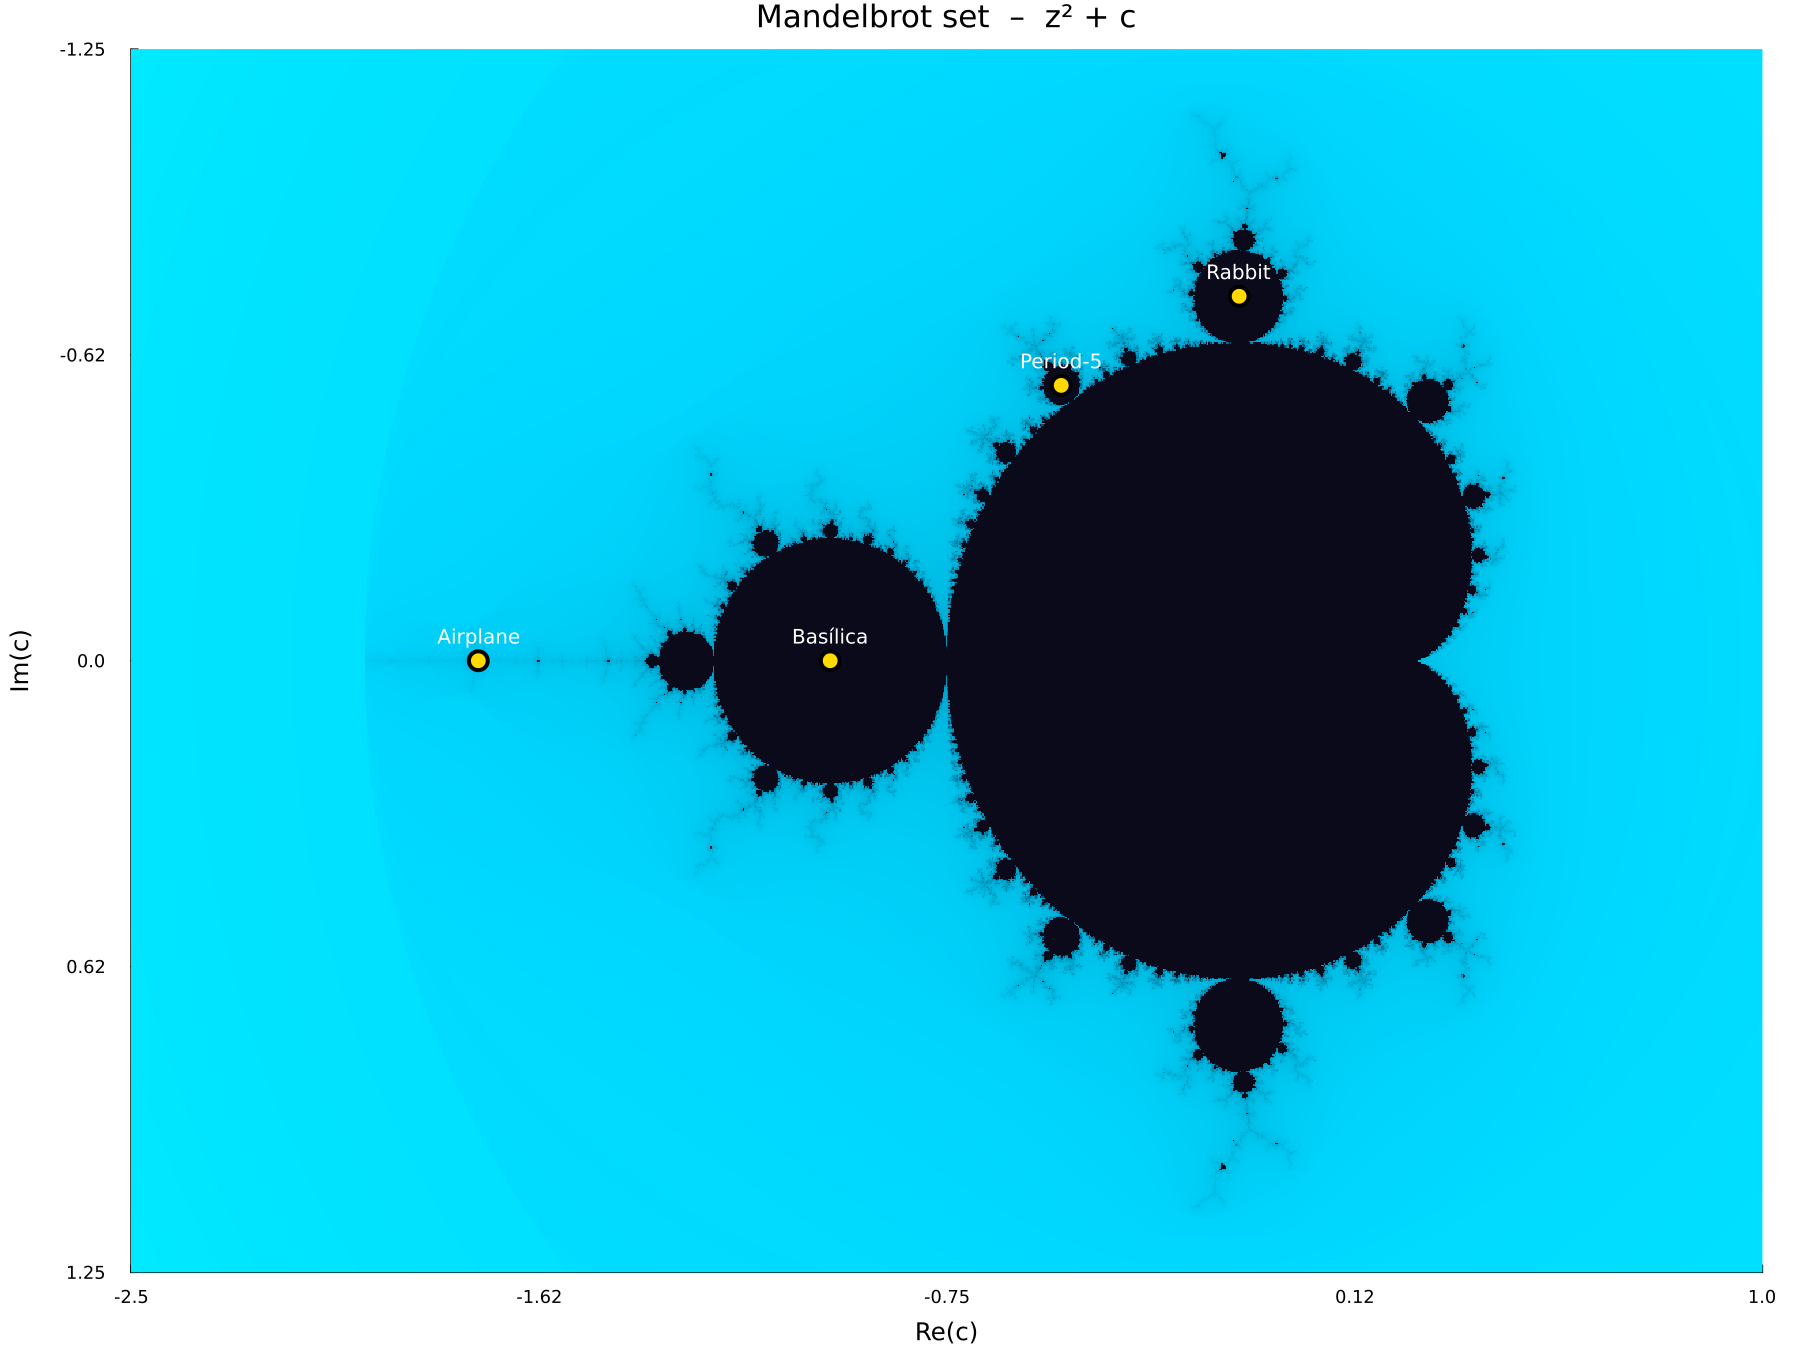
\includegraphics[width=0.80\textwidth]{figures/mandelbrot_portrait.png}
  \caption{The Mandelbrot set $\mathcal{M}$ rendered by
           \texttt{mandelbrot\_portrait} in
           \texttt{RiemannBasins.jl}.  The interior is shown in
           near-black; the exterior is shaded by normalised escape time
           \eqref{eq:escape_time} (blue gradient).
           The four centres of Table~\ref{tab:mandelbrot_centres} are
           marked with yellow dots: Bas\'ilica ($c=-1$), Airplane
           ($c\approx -1.7549$), Douady rabbit
           ($c\approx -0.1226+0.7449i$), and Period-$5$ centre
           ($c\approx -0.5043+0.5628i$).  Every marked point is a
           superattracting parameter; the corresponding Julia-set
           basin portraits are shown in
           Sections~\ref{subsec:basilica}--\ref{subsec:period5}.}
  \label{fig:mandelbrot_portrait}
\end{figure}

\begin{theorem}[Douady--Hubbard, 1982 \cite{DouadyHubbard1985}]
\label{thm:connectivity}
For the quadratic family $f_c(z)=z^2+c$, the following are equivalent:
\begin{enumerate}[label=\emph{(\roman*)}]
  \item The Julia set $J_c$ is connected.
  \item The filled Julia set $K_c=\{z\in\C : \{f_c^n(z)\}_{n\ge 0}
        \text{ is bounded}\}$ is connected.
  \item The critical orbit $\{0,c,c^2+c,\ldots\}$ is bounded, i.e.\
        $c\in\mathcal{M}$.
\end{enumerate}
If $c\notin\mathcal{M}$, then $J_c$ is a Cantor set and every immediate
basin is simply connected (in fact, $K_c=J_c$).
\end{theorem}

\begin{proof}[Proof idea]
The key tool is the \emph{B\"ottcher coordinate at $\infty$}: since
$\infty$ is a superattracting fixed point of $f_c$, there exists a
conformal map $\Phi_c\colon B^0_\infty\to\{|w|>1\}$ conjugating $f_c$ to
$w\mapsto w^2$.  The map $\Phi_c$ extends to the boundary of $B^0_\infty$
if and only if no critical value lies in $B^0_\infty$, i.e.\ $0\notin
B^0_\infty$, i.e.\ $c\in\mathcal{M}$.  When $c\in\mathcal{M}$, $\Phi_c$
extends to $\partial B^0_\infty=J_c$, showing $J_c$ is connected.  When
$c\notin\mathcal{M}$, $0\in B^0_\infty$ and iterating the Böttcher coordinate
shows $J_c$ is a Cantor set.
\end{proof}

All four examples of this article ($c=-1$, $c\approx-1.7549$,
$c\approx-0.1226+0.7449i$, $c\approx-0.5043+0.5628i$) lie inside
$\mathcal{M}$, so their Julia sets are connected and each immediate basin
$B^0_{z_k}$ is simply connected.  This is precisely what makes the
basin portraits of Figures~\ref{fig:basilica_pcycle}--\ref{fig:period5_lch}
consist of simply connected domains with no ``holes''.

\paragraph{External rays and the Green's function.}
The \emph{B\"ottcher coordinate at $\infty$} of $f_c$ defines the
\emph{Green's function}
\[
  G_c(z) = \lim_{n\to\infty} \frac{1}{2^n}\log|f_c^n(z)|,
  \qquad z\in B^0_\infty,
\]
which satisfies $G_c(f_c(z))=2G_c(z)$ and $G_c(z)\to 0$ as
$z\to\partial B^0_\infty=J_c$.  Level sets $\{G_c=r\}$ are
\emph{equipotential curves}; gradient lines of $G_c$ are the
\emph{external rays} $\mathcal{R}_c(\theta)$ (at angle $\theta\in[0,1)$).
When $c\in\mathcal{M}$, every rational ray $\mathcal{R}_c(p/q)$ lands
at a point of $J_c$ (Douady--Hubbard); the combinatorics of landing
points encodes the hyperbolic component structure of $\mathcal{M}$ and
connects the symbolic dynamics of angle-doubling to the topology of
$J_c$.  The normalised escape time~\eqref{eq:escape_time} is precisely
$G_c(c)/\log 2$ (up to additive normalisation), so the smooth colouring
of the exterior in Figure~\ref{fig:mandelbrot_portrait} is an approximation
of the Green's function, and the visible ``bands'' before smoothing are
the equipotential curves.

\subsection{The quadratic family $f_c(z)=z^2+c$ (Bas\'ilica, $c=-1$)}
\label{subsec:basilica}

The map $f_{-1}(z)=z^2-1$ has degree $d=2$, so $2d-2=2$ critical points.
In homogeneous notation: $F(z,t) = z^2-t^2$, $G(z,t)=t^2$.
The affine Wronskian is $W(z)=p'q-pq'=2z$, with unique root $z_0=0$.
Since $\deg W=1<2$, the point $\infty=[1:0]$ is also critical.

In the second chart $w=1/z$, $g(w)=w^2/(1-w^2)$ and $g'(0)=0$, so
$\infty$ is a \emph{superattracting} fixed point of $f_{-1}$.

The orbit of the finite critical point $z_0=0$:
\[
  0\;\overset{f}{\longmapsto}\;-1\;\overset{f}{\longmapsto}\;0
  \;\overset{f}{\longmapsto}\;-1\;\longmapsto\;\cdots
\]
This reveals the \emph{bas\'ilica 2-cycle} $\Gamma_2=\{0,-1\}$.  Since
$z_0=0\in\Gamma_2$ and $f'(0)=0$, the cycle is superattracting with $c=0$.
By Algorithm~\ref{alg:critical}, $P=2$.

The two basins $B_0$ and $B_{-1}$ partition the Fatou set (minus the
basin of $\infty$) into two equal components; their common boundary is
the bas'ilica Julia set, a dendrite-like connected curve
(see Figure~\ref{fig:basilica_pcycle}).

\begin{example}[Bas\'ilica computation]\label{ex:basilica}
\begin{verbatim}
  using RiemannBasins
  num = complex([-1.0, 0.0, 1.0]);  den = complex([1.0])
  print_critical_orbit_summary(num, den)
  # → P = 2 (superattracting 2-cycle, c = 0.0)
  basin_portrait_pcycle(num, den, 2; iter=400, show_plot=true)
\end{verbatim}
\end{example}

\begin{figure}[htbp]
  \centering
  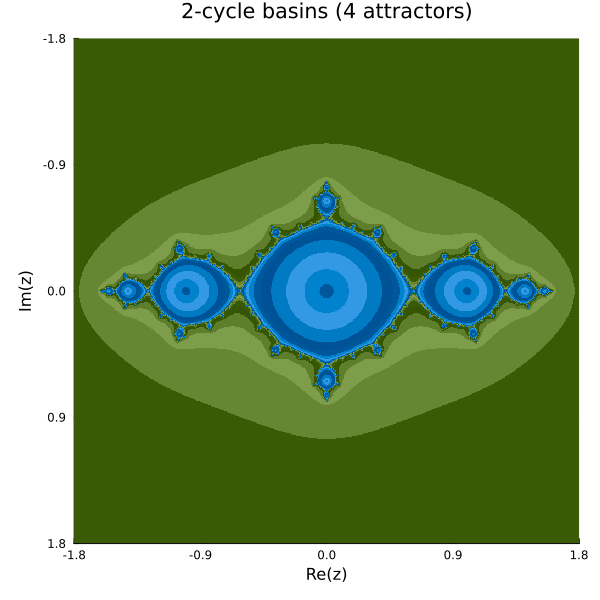
\includegraphics[width=0.65\textwidth]{figures/pcycle_basilica_2cycle.png}
  \caption{Basin portrait of the 2-cycle of $f_{-1}(z)=z^2-1$ (bas\'ilica).
           Each colour represents the basin of one element of the
           superattracting 2-cycle $\{0,-1\}$; the grey region is the
           basin of $\infty$.}
  \label{fig:basilica_pcycle}
\end{figure}

Figure~\ref{fig:basilica_pcycle} follows the classical convention: each
colour is assigned to one \emph{orbit group}, so both sub-basins of the
same cycle share a common hue family.  The \texttt{pcycle\_lch} strategy
of Section~\ref{sec:colour} goes one step further and encodes which
sub-basin each pixel belongs to via a hue shift $\Delta H$.
For $p=2$ with \texttt{hue\_band}$=120^\circ$ the two sub-basins
$B_0\ni 0$ and $B_{-1}\ni -1$ are separated by $60^\circ$ within the
same perceptual hue family, making the cyclic permutation
$f\colon B_0\to B_{-1}\to B_0$ directly readable from the image
(Figure~\ref{fig:basilica_pcycle_lch}).

\begin{figure}[htbp]
  \centering
  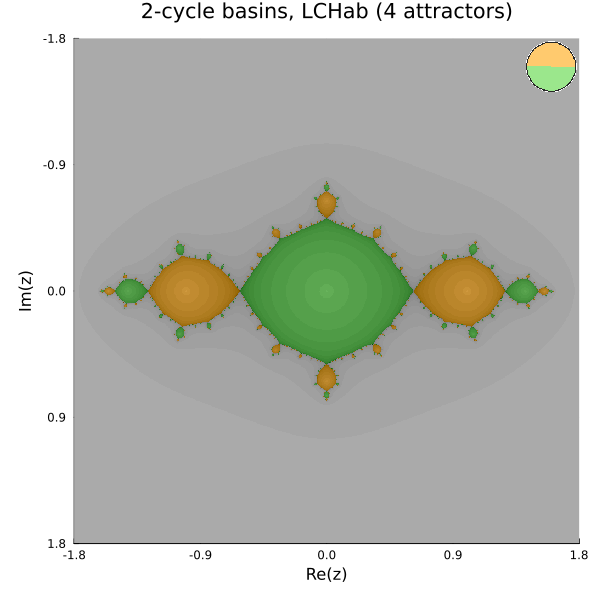
\includegraphics[width=0.65\textwidth]{figures/pcycle_basilica_2cycle_lch.png}
  \caption{The same map $f_{-1}(z)=z^2-1$ rendered with the
           \texttt{pcycle\_lch} strategy (\texttt{hue\_band}$=120^\circ$).
           The two sub-basins $B_0$ (lighter hue) and $B_{-1}$ (darker hue)
           are now distinguished by a $60^\circ$ hue shift; their
           common boundary is the bas\'ilica Julia set.}
  \label{fig:basilica_pcycle_lch}
\end{figure}


\subsection{Newton's method for $z^3-1$}

Newton's method $N(z)=\frac{2z^3+1}{3z^2}$ has degree $d=3$.
The Wronskian $W(z)=6z^2\cdot 3z^2 - (2z^3+1)\cdot 6z = 6z(z^3-1)$.
The four critical points are $z=0$ and $z\in\{1,\omega,\bar\omega\}$
where $\omega=e^{2\pi i/3}$.

The three roots of unity are superattracting fixed points of $N$ (Newton
converges quadratically).  The critical point $z=0$ maps to
$N(0)=\infty$; in the second chart $g(w)=3w/(2+w^3)$, $g'(0)=3/2>1$,
so $\infty$ is \emph{repelling} and the orbit of $z=0$ is
\emph{indeterminate}.

The three superattracting fixed points give $P=1$ (see Figure~\ref{fig:newton_z3_pcycle}).

\begin{example}[Newton portrait]
\begin{verbatim}
  num = complex([1.0, 0.0, 0.0, 2.0])
  den = complex([0.0, 0.0, 3.0, 0.0])
  print_critical_orbit_summary(num, den)
  # → 3 superattracting fixed points (p=1), 1 indeterminate
  # → P = 1
  basin_portrait_pcycle(num, den, 1; iter=300, show_plot=true)
\end{verbatim}
\end{example}

\begin{figure}[htbp]
  \centering
  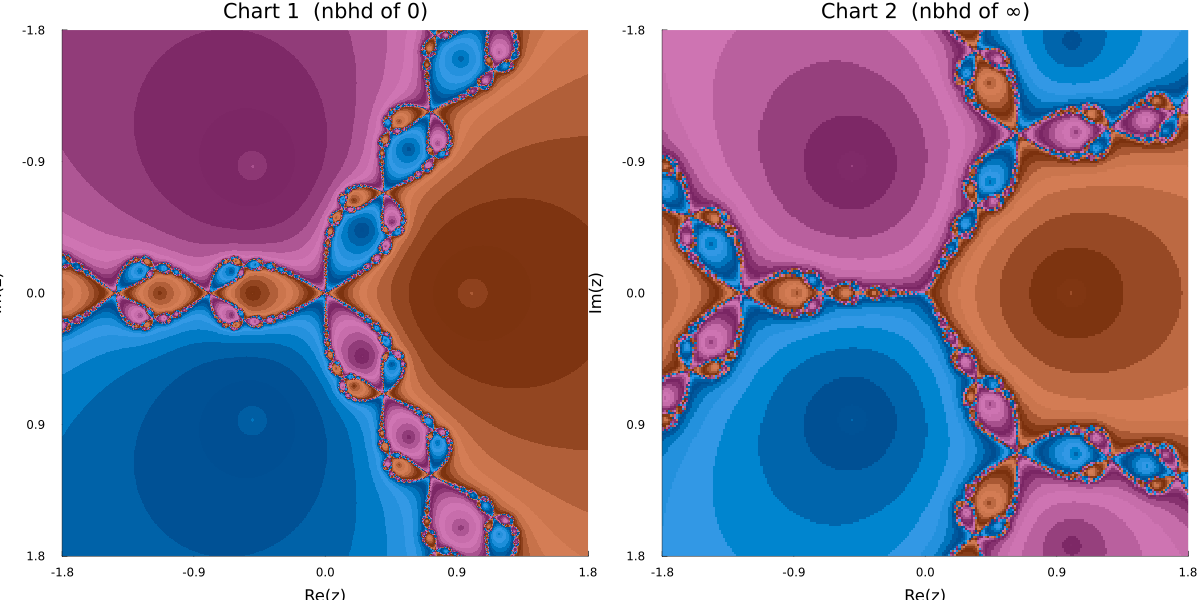
\includegraphics[width=0.90\textwidth]{figures/pcycle_newton_z3.png}
  \caption{Basin portrait of Newton's method for $z^3-1$ in both affine
           charts of $\Pone$.  Chart~1 (left) shows the neighbourhood of
           the origin; Chart~2 (right) the neighbourhood of $\infty$.
           The three superattracting fixed points (roots of $z^3-1$) each
           attract a connected basin; $\infty$ is repelling.}
  \label{fig:newton_z3_pcycle}
\end{figure}


\subsection{Halley's method for $z^3-1$}
\label{subsec:halley}

Halley's method (1694) for solving $p(z)=0$ is the second-order
Householder iteration
\begin{equation}\label{eq:halley}
  H(z) = z - \frac{2p(z)p'(z)}{2[p'(z)]^2 - p(z)p''(z)}.
\end{equation}
It achieves \emph{cubic} convergence near a simple root (error cubed at
each step), compared with quadratic for Newton.

\paragraph{Rational form for $p(z)=z^3-1$.}
With $p(z)=z^3-1$, $p'(z)=3z^2$, $p''(z)=6z$ formula~\eqref{eq:halley} simplifies to
\begin{equation}\label{eq:halley_z3}
  H(z) = \frac{z(z^3+2)}{2z^3+1}
        = \frac{z^4+2z}{2z^3+1},
\end{equation}
a rational map of degree $d=4$.  The Wronskian (in the affine chart) is
\[
  W(z) = P'Q - PQ'
       = (4z^3+2)(2z^3+1)-(z^4+2z)(6z^2)
       = 2(z^3-1)^2 = 2(z-1)^2(z-\omega)^2(z-\bar\omega)^2,
\]
where $\omega=e^{2\pi i/3}$.  Thus $H$ has $2d-2=6$ critical points
(counted with multiplicity), all coinciding with the three roots of unity
$1,\omega,\bar\omega$, each of multiplicity~$2$.

\paragraph{Fixed-point analysis.}
The fixed points of $H$ are found by solving $H(z)=z$:
\[
  z(z^3+2) = z(2z^3+1) \;\Longrightarrow\; z^3=1
  \quad\text{(plus }z=0\text{ and }z=\infty\text{)}.
\]
So $H$ has five fixed points in $\Pone$ ($=d+1$):
\begin{itemize}
  \item $z=1,\omega,\bar\omega$: superattracting (each is both a critical
        point and a fixed point, so the multiplier $H'(z_k)=0$).
  \item $z=0$: repelling, $H'(0)=2(0-1)^2/(2\cdot 0+1)^2=2$.
  \item $z=\infty$: repelling (in the second chart
        $\hat H(w)=w(2+w^3)/(1+2w^3)$, $\hat H'(0)=2$).
\end{itemize}
Since every critical point lies in an immediate basin of a superattracting
fixed point, Fatou's theorem gives $P=1$ and the dynamics is completely
determined by the three basins.

The convergence near the roots is cubic rather than quadratic, which
manifests in the basin portrait as smoother boundaries and a steeper
lightness gradient away from each attractor.  Compare
Figure~\ref{fig:halley_z3_pcycle} with the Newton portrait
(Figure~\ref{fig:newton_z3_pcycle}): the basins are qualitatively similar
but the Julia set of Halley is strictly contained in that of Newton's
method (Halley converges for strictly more starting points), and the
interior shading is more compressed near the attractors.

\begin{example}[Halley portrait]
\begin{verbatim}
  # H(z) = (z^4+2z)/(2z^3+1)
  num = complex([0.0, 2.0, 0.0, 0.0, 1.0])   # z^4 + 2z
  den = complex([1.0, 0.0, 0.0, 2.0])         # 2z^3 + 1
  print_critical_orbit_summary(num, den)
  # → 3 superattracting fixed points (p=1), 2 repelling fixed points
  # → P = 1
  basin_portrait_pcycle(num, den, 1; iter=300, colorstrategy="pcycle_lch",
                        show_plot=true)
\end{verbatim}
\end{example}

\begin{figure}[htbp]
  \centering
  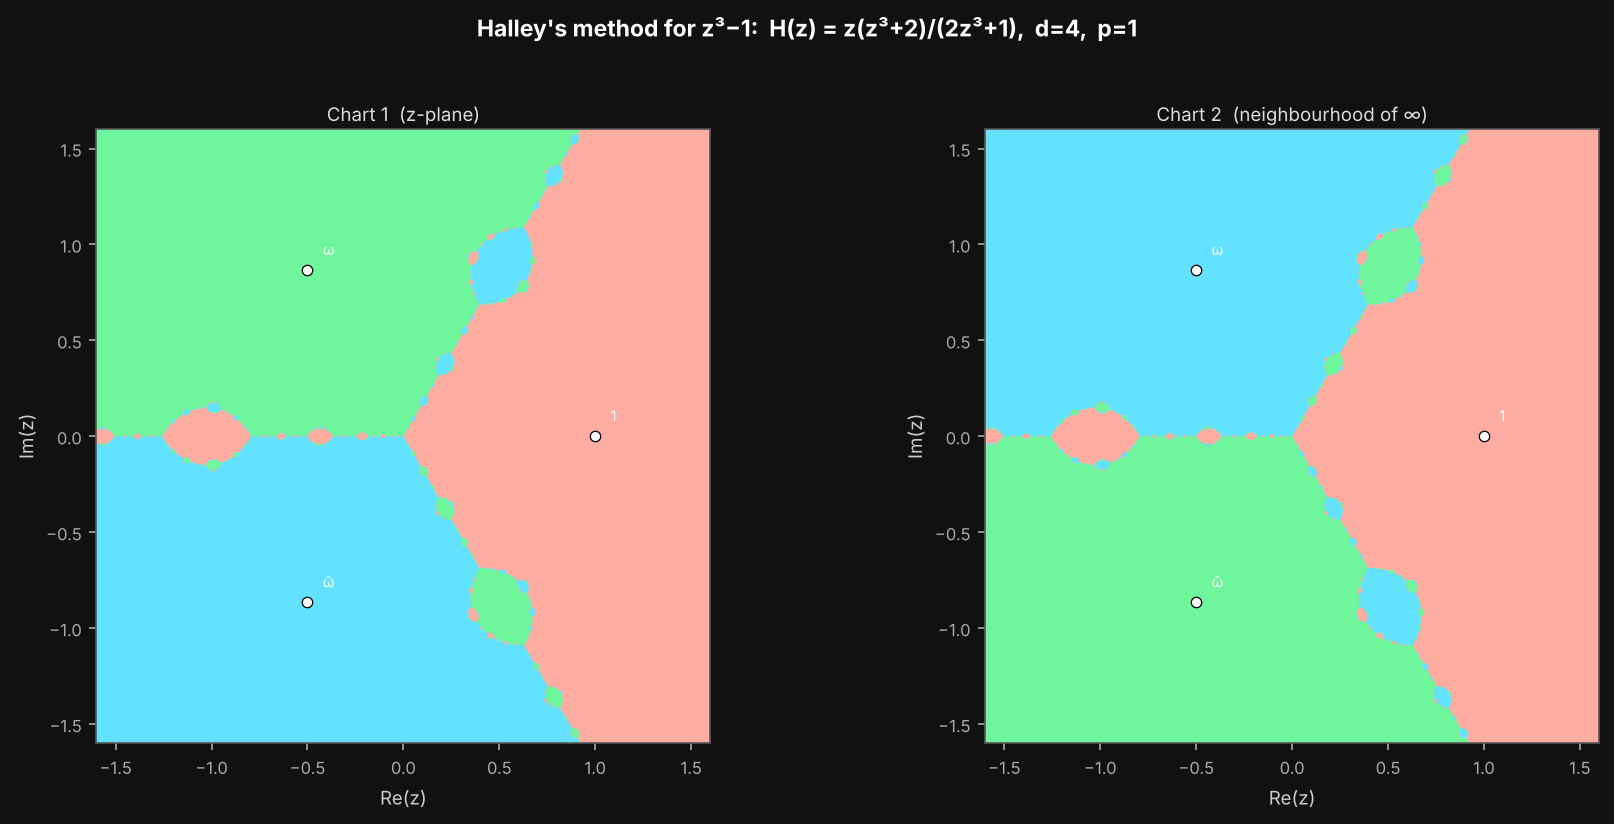
\includegraphics[width=0.90\textwidth]{figures/pcycle_halley_z3.png}
  \caption{Basin portrait of Halley's method~\eqref{eq:halley_z3} for
           $z^3-1$, $d=4$.  Three superattracting fixed points
           $1,\omega,\bar\omega$ (roots of $z^3-1$) each of multiplicity~2;
           two repelling fixed points at $z=0$ and $z=\infty$.
           Compare with Figure~\ref{fig:newton_z3_pcycle}: Halley's
           basins cover a larger portion of the sphere.}
  \label{fig:halley_z3_pcycle}
\end{figure}

\subsection{The map $f(z)=z^2$ (superattracting fixed point)}

For $f(z)=z^2$: $W(z)=2z$, unique critical point $z=0$, orbit $0\to 0$.
Since $f'(0)=0$, $c=0$ and $P=1$.  The basin of $0$ is the open unit disc
$\{|z|<1\}$ and the Julia set is the unit circle $\{|z|=1\}$ (see Figure~\ref{fig:z2_fixed}).

\begin{figure}[htbp]
  \centering
  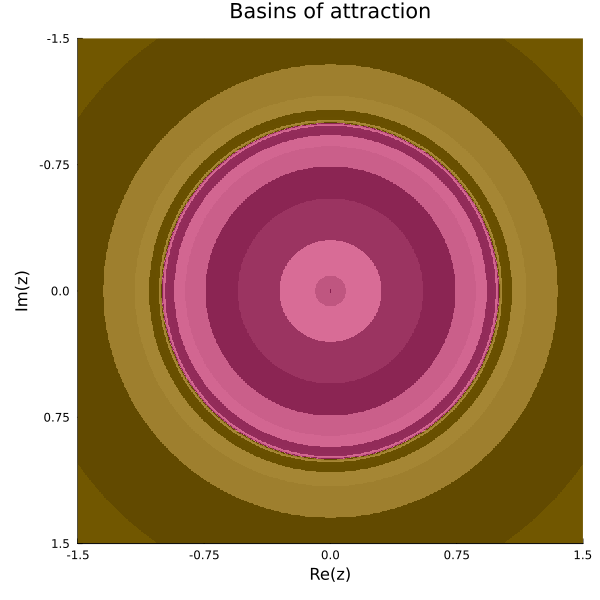
\includegraphics[width=0.55\textwidth]{figures/pcycle_z2_fixed.png}
  \caption{Basin portrait of $f(z)=z^2$.  The open unit disc $\{|z|<1\}$
           (blue) is the basin of the superattracting fixed point $z=0$;
           the exterior $\{|z|>1\}$ is the basin of $\infty$.
           The unit circle $\{|z|=1\}$ is the Julia set.}
  \label{fig:z2_fixed}
\end{figure}

\subsection{The airplane map $f_c(z)=z^2+c$ (3-cycle, $c\approx-1.7549$)}
\label{subsec:airplane}

The map $f_c(z)=z^2+c$ with $c$ the unique real root of
\[
  c^3+2c^2+c+1=0, \qquad c\approx -1.7549,
\]
has degree $d=2$ and a single finite critical point $z_0=0$ (Wronskian $W(z)=2z$).
Evaluating:
\[
  f_c(0)=c, \quad f_c(c)=c^2+c, \quad f_c(c^2+c)=(c^2+c)^2+c=0,
\]
where the last equality holds precisely because $c$ satisfies $c^3+2c^2+c+1=0$.
Hence $0$ lies on a \emph{superattracting 3-cycle}
$\Gamma_3=\{0,\,c,\,c^2+c\}$, and Algorithm~\ref{alg:critical} returns $P=3$
(see Figure~\ref{fig:airplane_pcycle}).

The corresponding Julia set---known as the \emph{airplane}---is a connected,
locally connected compact set with a characteristic ``airplane wing'' shape.
The Fatou set decomposes into three basins $B_0$, $B_c$, $B_{c^2+c}$, one for
each element of the 3-cycle, together with the basin of $\infty$.

\begin{example}[Airplane computation]
\begin{verbatim}
  using RiemannBasins
  # c is the real root of c^3 + 2c^2 + c + 1 = 0
  c = let x = -1.75
        for _ in 1:50; x -= (x^3+2x^2+x+1)/(3x^2+4x+1) end; x
      end
  num = complex([c, 0.0, 1.0]);  den = complex([1.0])
  print_critical_orbit_summary(num, den)
  # → P = 3 (superattracting 3-cycle, c = 0.0)
  basin_portrait_pcycle(num, den, 3; iter=400, show_plot=true)
\end{verbatim}
\end{example}

\begin{figure}[htbp]
  \centering
  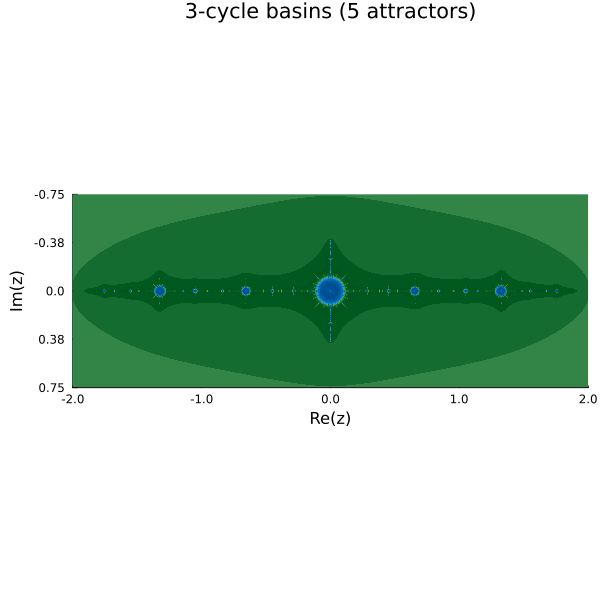
\includegraphics[width=0.80\textwidth]{figures/pcycle_airplane_3cycle.png}
  \caption{Basin portrait of the 3-cycle of the airplane map
           $f_c(z)=z^2+c$ ($c\approx-1.7549$, the real root of
           $c^3+2c^2+c+1=0$).  The three colours correspond to the
           basins of $B_0$, $B_c$ and $B_{c^2+c}$; grey is the
           basin of $\infty$.  The bounded components of the Fatou
           set form the characteristic ``airplane'' shape.}
  \label{fig:airplane_pcycle}
\end{figure}


\subsection{The Douady rabbit $f_c(z)=z^2+c$ (3-cycle, $c\approx-0.1226+0.7449i$)}
\label{subsec:rabbit}

The same polynomial equation
\[
  c^3+2c^2+c+1=0
\]
that determines the airplane parameter (Section~\ref{subsec:airplane}) has
two additional complex conjugate roots.  Taking the root with positive
imaginary part gives
\[
  c_{\mathrm{r}}\approx -0.12256116688 + 0.74486176662i,
\]
the parameter of the \emph{Douady rabbit} \cite{DouadyHubbard1985}.  Since
$c_{\mathrm{r}}$ satisfies the same equation, the critical orbit verification
is identical:
\[
  f_{c_{\mathrm{r}}}(0)=c_{\mathrm{r}},\quad
  f_{c_{\mathrm{r}}}(c_{\mathrm{r}})=c_{\mathrm{r}}^2+c_{\mathrm{r}},\quad
  f_{c_{\mathrm{r}}}(c_{\mathrm{r}}^2+c_{\mathrm{r}})=0,
\]
so $0$ lies on a superattracting 3-cycle
$\Gamma_3=\{0,\,c_{\mathrm{r}},\,c_{\mathrm{r}}^2+c_{\mathrm{r}}\}$ and
Algorithm~\ref{alg:critical} returns $P=3$ as for the airplane.

Geometrically the two maps are strikingly different.  The airplane Julia set
has thin antenna-like tendrils; the Douady rabbit Julia set is a connected,
locally connected compact set with three prominent \emph{round petals}---the
visual origin of its name \cite{DouadyHubbard1985}.  These large, rounded
sub-basins make the rabbit a cleaner illustration of the
\texttt{pcycle\_lch} colour encoding: with
\texttt{hue\_band}$=120^\circ$ each of the three sub-basins $B_0$,
$B_{c_{\mathrm{r}}}$, $B_{c_{\mathrm{r}}^2+c_{\mathrm{r}}}$ receives a
hue offset of $40^\circ$ within the same perceptual hue family, producing
three clearly distinguishable shades
(see Figure~\ref{fig:rabbit_pcycle_lch}).

\begin{example}[Douady rabbit with LCH coloring]
\begin{verbatim}
  using RiemannBasins
  # c is the complex root of c^3 + 2c^2 + c + 1 = 0, Im(c) > 0
  c_rabbit = let x = complex(-0.12, 0.75)
               for _ in 1:80
                 x -= (x^3 + 2x^2 + x + 1) / (3x^2 + 4x + 1)
               end; x
             end
  num = ComplexF64.([c_rabbit, 0.0, 1.0])
  den = ComplexF64.([1.0])
  basin_portrait_pcycle(num, den, 3;
                        iter = 400,
                        colorstrategy = "pcycle_lch",
                        hue_band = 120.0,
                        show_cyclic_palette = true,
                        xinterval = (-1.5, 1.5),
                        yinterval = (-1.5, 1.5))
\end{verbatim}
\end{example}

\begin{figure}[htbp]
  \centering
  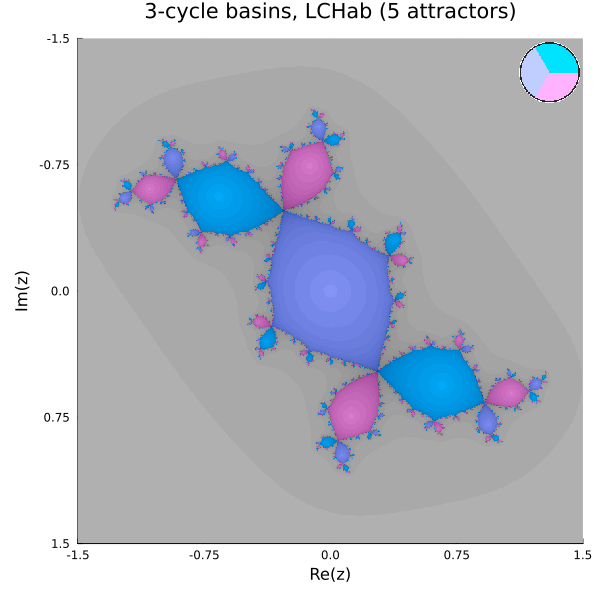
\includegraphics[width=0.70\textwidth]{figures/pcycle_rabbit_3cycle_lch.png}
  \caption{Basin portrait of the Douady rabbit $f_c(z)=z^2+c$
           ($c\approx -0.1226+0.7449i$, the complex root with positive
           imaginary part of $c^3+2c^2+c+1=0$)
           rendered with the \texttt{pcycle\_lch} colour strategy
           (\texttt{hue\_band}$=120^\circ$).
           The three sub-basins $B_0$, $B_{c_{\mathrm{r}}}$,
           $B_{c_{\mathrm{r}}^2+c_{\mathrm{r}}}$ are separated by
           hue offsets of $40^\circ$; grey is the basin of~$\infty$.
           Compared with the airplane (Figure~\ref{fig:airplane_pcycle}),
           the sub-basins are large and round, making the cyclic permutation
           $f\colon B_0\to B_{c_{\mathrm{r}}}\to
           B_{c_{\mathrm{r}}^2+c_{\mathrm{r}}}\to B_0$
           directly readable from the colours.}
  \label{fig:rabbit_pcycle_lch}
\end{figure}

%% ---------------------------------------------------------------------------
\subsection{Period-5 centre $f_c(z)=z^2+c$
            ($c\approx-0.5043+0.5628i$, 5-cycle)}
\label{subsec:period5}
%% ---------------------------------------------------------------------------

The Mandelbrot set contains a hyperbolic component of period~5 attached to
the main cardioid at internal angle $1/5$.  Its centre satisfies
$f_c^{\circ 5}(0)=0$ and is located at
\[
  c_5\approx -0.50434017545 + 0.56276576145i.
\]
For this parameter the critical orbit closes after exactly five steps, so
Algorithm~\ref{alg:critical} returns $P=5$.

The five sub-basins $B_0,B_1,\ldots,B_4$ (indexed by the position of a
pixel's limit point in $\Gamma_5$) are related by the cyclic permutation
$f\colon B_k\to B_{k+1\bmod 5}$.  With \texttt{hue\_band}$=150^\circ$
the encoding assigns hue offsets $0^\circ,30^\circ,60^\circ,90^\circ,
120^\circ$ to $B_0,\ldots,B_4$, yielding five perceptually well-separated
shades within a single Okabe-Ito hue family
(see Figure~\ref{fig:period5_lch}).  The image reveals the five-fold
rotational near-symmetry of the Julia set and makes the cyclic dynamics
directly legible at a glance.  The circular colour-wheel inset in the
top-right corner displays the five sub-basin hues in cyclic order
($B_0\to B_1\to\cdots\to B_4\to B_0$), serving as an on-figure legend
for the colour encoding.

\begin{example}[Period-5 centre]
\begin{verbatim}
  using RiemannBasins
  c5 = let x = complex(-0.5024, 0.5629)
         for _ in 1:100
           z = 0+0im; dz = 0+0im
           for _ in 1:5
             z, dz = z^2 + x, 2z*dz + 1
           end
           x -= z/dz
         end; x
       end   # = -0.50434...+0.56277...i
  num = ComplexF64.([c5, 0.0, 1.0])
  den = ComplexF64.([1.0])
  basin_portrait_pcycle(num, den, 5;
                        iter = 500,
                        colorstrategy = "pcycle_lch",
                        hue_band = 150.0,
                        show_cyclic_palette = true,
                        xinterval = (-1.5, 1.6),
                        yinterval = (-1.2, 1.9))
\end{verbatim}
\end{example}

\begin{figure}[htbp]
  \centering
  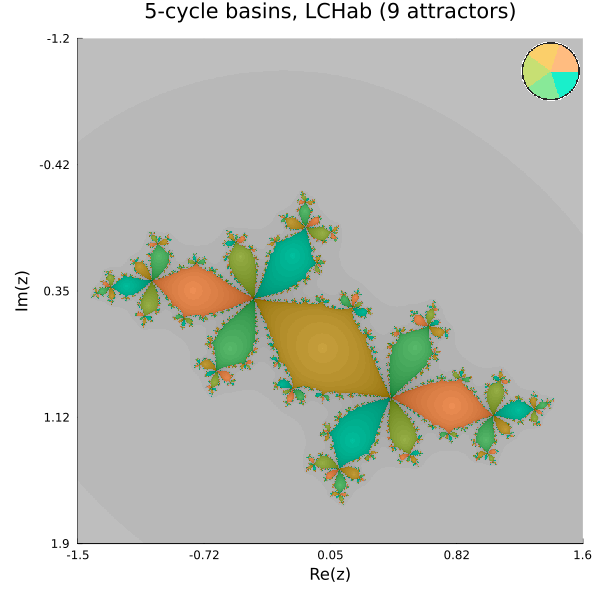
\includegraphics[width=0.70\textwidth]{figures/pcycle_period5_lch.png}
  \caption{Basin portrait of the period-5 centre
           $f_c(z)=z^2+c$ ($c\approx-0.5043+0.5628i$, superattracting
           5-cycle) with the \texttt{pcycle\_lch} colour strategy
           (\texttt{hue\_band}$=150^\circ$, hue step $30^\circ$ per
           sub-basin).  The five sub-basins $B_0,\ldots,B_4$ are encoded
           by increasing hue within the same perceptual family; the
           five-fold near-symmetry of the Julia set and the cyclic
           permutation $f\colon B_0\to B_1\to\cdots\to B_4\to B_0$
           are readable directly from the colour progression.
           The circular colour-wheel inset (top right) shows the five
           sub-basin hues in their cyclic order.}
  \label{fig:period5_lch}
\end{figure}

\subsection{A proper rational map: $f(z)=(z^2-1)/(z^2+1)$}
\label{subsec:rational}

All preceding examples are either polynomials or related to root-finding
iteration.  We now exhibit a \emph{genuinely rational} function whose
dynamics is not conjugate to any polynomial---here both $0$ and $\infty$
play symmetric roles---and that has a superattracting $2$-cycle.

\paragraph{The map and its critical points.}
Set $f(z)=(z^2-1)/(z^2+1)$, a rational map of degree $d=2$.
The Wronskian (affine chart) is
\[
  W(z) = P'Q - PQ' = 2z(z^2+1) - (z^2-1)2z = 4z,
\]
so the only affine critical point is $z=0$ (with multiplicity~1); the
second critical point is $z=\infty$ (Wronskian degree $=2d-2=2$). 

\paragraph{Superattracting 2-cycle.}
Direct calculation gives
\[
  f(0) = \frac{0-1}{0+1} = -1, \qquad f(-1) = \frac{1-1}{1+1} = 0,
\]
so $\{0,-1\}$ is a $2$-cycle.  Since $f'(0)=4\cdot 0/(0+1)^2=0$, the
cycle point $z_0=0$ is a critical point; hence $\{0,-1\}$ is a
\emph{superattracting} $2$-cycle (Lyapunov constant $c(\{0,-1\})=0$).

The orbit of the second critical point: $f(\infty)=1$, $f(1)=0$, and
from that point on the orbit follows the $2$-cycle.  Thus \emph{both}
critical points are attracted to $\{0,-1\}$, confirming by
Corollary~\ref{cor:bound} that this is the \emph{only} attracting cycle
and $P=2$.

\paragraph{Fixed points.}
Solving $f(z)=z$ gives $z^3-z^2+z+1=0$, whose three solutions are all
repelling (since both critical orbits converge to the $2$-cycle, there
is no critical point available to stabilize a fixed point).

\begin{example}[Proper rational portrait]
\begin{verbatim}
  # f(z) = (z^2 - 1) / (z^2 + 1)
  num = complex([-1.0, 0.0, 1.0])   # z^2 - 1
  den = complex([ 1.0, 0.0, 1.0])   # z^2 + 1
  print_critical_orbit_summary(num, den)
  # → 1 superattracting 2-cycle, 3 repelling fixed points
  # → P = 2
  basin_portrait_pcycle(num, den, 2; iter=400, colorstrategy="pcycle_lch",
                        hue_band=180.0, show_plot=true)
\end{verbatim}
\end{example}

\begin{figure}[htbp]
  \centering
  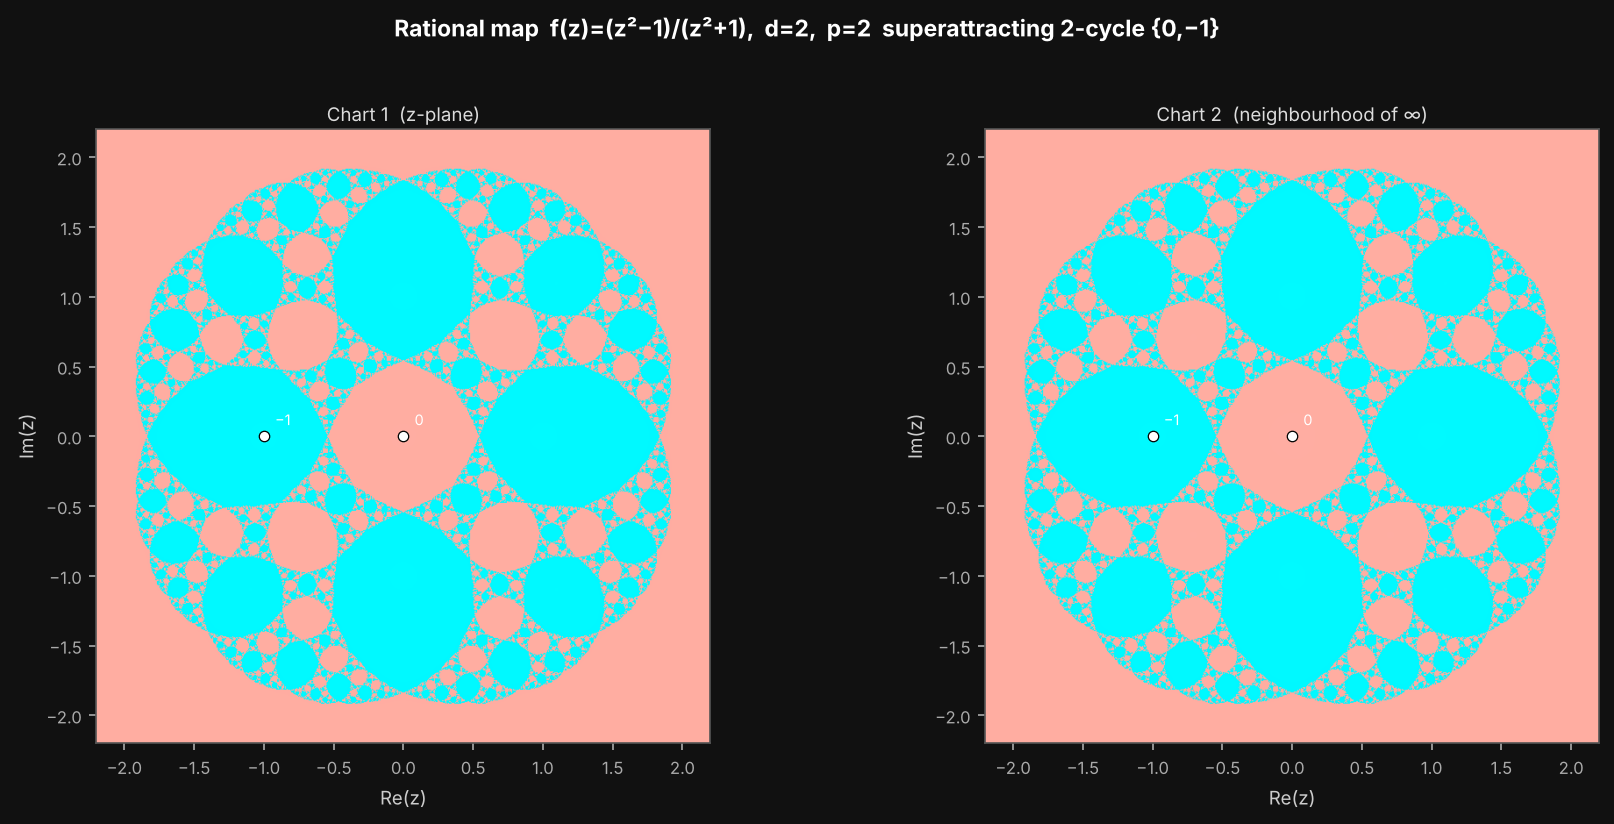
\includegraphics[width=0.90\textwidth]{figures/pcycle_rational_2cycle.png}
  \caption{Basin portrait of $f(z)=(z^2-1)/(z^2+1)$, the simplest
           proper rational map with a superattracting $2$-cycle $\{0,-1\}$.
           Degree $d=2$, two critical points ($z=0$ and $z=\infty$), both
           attracted to the cycle.  Chart~1 (left): the two immediate basins
           $B^0_0$ (orange) and $B^0_{-1}$ (blue) separated by the Julia set.
           Chart~2 (right): the neighbourhood of $\infty$, which lies in
           $B^0_0$ since $\infty\to 1\to 0$.}
  \label{fig:rational_2cycle}
\end{figure}

\subsection{Summary table}

\begin{center}
\begin{tabular}{lcccc}
\toprule
Map & $d$ & $\#$ crit.\ pts & $P$ & Dominant labels\\
\midrule
M\"obius (degree 1)  & 1 & 0  & 0 & --- \\
$f(z)=z^2$         & 2 & 1  & 1 & superattr.\ ($p=1$) \\
$f(z)=z^2-1$       & 2 & 2  & 2 & superattr.\ ($p=2$) + superattr.\ ($p=1$ at $\infty$) \\
Newton $z^3-1$     & 3 & 4  & 1 & 3 superattr.\ ($p=1$) + 1 indet. \\
Airplane $z^2+c$   & 2 & 2  & 3 & superattr.\ ($p=3$) + superattr.\ ($p=1$ at $\infty$) \\
Rabbit $z^2+c$     & 2 & 2  & 3 & superattr.\ ($p=3$) + superattr.\ ($p=1$ at $\infty$) \\
Period-5 $z^2+c$   & 2 & 2  & 5 & superattr.\ ($p=5$) + superattr.\ ($p=1$ at $\infty$) \\
Halley $z^3-1$     & 4 & 6  & 1 & 3 superattr.\ ($p=1$), 2 repelling fixed pts \\
$(z^2-1)/(z^2+1)$  & 2 & 2  & 2 & 1 superattr.\ $2$-cycle (proper rational) \\
\bottomrule
\end{tabular}
\end{center}

%% ===========================================================================
\section{Discussion and open problems}
\label{sec:discussion}
%% ===========================================================================

\subsection{The bound $P$ and its sharpness}

By Corollary~\ref{cor:complete}, the bound $P$ output by
\texttt{max\_attracting\_period} is sharp: there is no attracting cycle
of period $>P$.  However, $P$ is computed via a finite warmup (default
$N_{\mathrm{warm}}=300$), so if the warmup is insufficient for a
slowly-converging attracting cycle, $P$ may be underestimated.
A conservative use of the bound requires checking that the
Lyapunov constant satisfies $c\ll 1$; near a parabolic
parameter where $c\to 1$, the warmup must be increased substantially.

\subsection{Beyond attracting cycles}

The current algorithms detect only attracting and superattracting cycles.
Parabolic cycles ($|\lambda|=1$, $\lambda^q=1$) also attract orbits, but
at polynomial rather than exponential rate; they require a modified
detection scheme based on Fatou coordinates.  Siegel discs and Herman
rings require a different approach (e.g., measuring the autocorrelation
of the orbit to detect irrational rotation numbers).

\subsection{Families and bifurcations}

For a one-parameter family $f_c$ (e.g., $z^2+c$),
the function $c\mapsto P(c)$ records the attracting period.  Its level
sets are the \emph{hyperbolic components} of the Mandelbrot set
$\mathcal{M}$ (Section~\ref{subsec:mandelbrot}, \cite{DouadyHubbard1985}):
$P(c)=p$ on the interior of $H_p$, while $P(c)=0$ on the exterior
of $\mathcal{M}$ (escaping parameters) and on the boundary
$\partial\mathcal{M}$ (parabolic, Siegel, Misiurewicz and other
non-hyperbolic parameters).

The Mandelbrot portrait produced by \texttt{mandelbrot\_portrait}
(Figure~\ref{fig:mandelbrot_portrait}) can therefore be read as a
\emph{parameter portrait}: each pixel colour encodes the escape speed
of the critical orbit, and the near-black interior is exactly
$\mathcal{M}$.  The four superattracting centres studied in this article
are marked explicitly on the figure; they are canonical representatives
of periods $2$, $3$, $3$, and $5$.

An algorithmic study of the hyperbolic boundaries of $\mathcal{M}$ via
\texttt{max\_attracting\_period} applied to a dense parameter grid is
a natural extension of the present work, and would yield a computational
counterpart to the theoretical description of $\mathcal{M}$ in
\cite{DouadyHubbard1985}.

\subsection{Algorithmic complexity and parallelism}

Both algorithms are embarrassingly parallel over grid points
(Algorithm~\ref{alg:basin}) and over critical points
(Algorithm~\ref{alg:critical}).  Julia's threading model and
GPU backends (via \texttt{CUDA.jl}) can accelerate the portrait
computation by several orders of magnitude for high-resolution images.

\subsection{Homogeneous arithmetic and exact computation}

For maps with algebraic coefficients, the Wronskian roots can in principle
be computed exactly (via resultant-based methods).  An exact
implementation would eliminate the deduplication tolerance in
Algorithm~\ref{alg:critical} and give a provably correct critical point
count.

%% ===========================================================================
\section{Conclusions}
\label{sec:conclusions}
%% ===========================================================================

We have presented a self-contained algorithmic framework for the computation
of basins of attraction of $p$-cyclic orbits of rational maps on the Riemann
sphere $\Pone$, based entirely on homogeneous coordinates and the chordal
metric.  The key contributions are:

\begin{enumerate}
  \item A two-chart formula for the spherical derivative $\fsh$
        (Proposition~\ref{prop:sphderiv}) that is correct at all points of
        $\Pone$, including $\infty=[1:0]$, correcting a subtle error in
        naive single-chart implementations (Remark~\ref{rem:chartbug}).

  \item Algorithm~\ref{alg:critical} (\texttt{critical\_orbit\_analysis})
        implementing Fatou's theorem to locate all attracting cycles and
        compute a sharp upper bound $P$ on the maximum attracting period.

  \item Algorithm~\ref{alg:basin} (\texttt{basin\_portrait\_pcycle})
        producing colour-coded basin portraits for any user-specified period
        $p$, with full support for the two-chart global portrait on $\Pone$.

  \item A suite of 94 automated tests in \texttt{RiemannBasins.jl}
        validating the algorithms on the quadratic family, Newton's method,
        and M\"obius transformations.
\end{enumerate}

The combination of Algorithms~\ref{alg:critical} and~\ref{alg:basin} gives a
principled workflow: run Algorithm~\ref{alg:critical} first to determine $P$,
then run Algorithm~\ref{alg:basin} only for $p\leq P$, avoiding unnecessary
computation.

\bigskip
\noindent\textbf{Acknowledgements.}
This work is a continuation of the program
initiated in \cite{Extremiana2019,AlvarezAparicio2023}.  Computations were
performed using the Julia language \cite{Julia2017} with the
\texttt{RiemannBasins.jl} package \cite{RiemannBasins}.
L.\,J.\,H.-P.\ acknowledges support from project REGI25/61 of the
Universidad de La Rioja.

%% ===========================================================================
\bibliographystyle{plain}
\bibliography{draft_pcycle_basins}
%% ===========================================================================

\end{document}
